% $Header: /Users/joseph/Documents/LaTeX/beamer/solutions/generic-talks/generic-ornate-15min-45min.en.tex,v 90e850259b8b 2007/01/28 20:48:30 tantau $

\documentclass[svgnames,smaller]{beamer}

% This file is a solution template for:

% - Giving a talk on some subject.
% - The talk is between 15min and 45min long.
% - Style is ornate.



% Copyright 2004 by Till Tantau <tantau@users.sourceforge.net>.
%
% In principle, this file can be redistributed and/or modified under
% the terms of the GNU Public License, version 2.
%
% However, this file is supposed to be a template to be modified
% for your own needs. For this reason, if you use this file as a
% template and not specifically distribute it as part of a another
% package/program, I grant the extra permission to freely copy and
% modify this file as you see fit and even to delete this copyright
% notice. 

\mode<presentation>
{
  \usetheme{Darmstadt}
 	\usecolortheme[named=ForestGreen]{structure}

  \setbeamercovered{transparent}
  % or whatever (possibly just delete it)
}


\usepackage[english]{babel}
% or whatever

\usepackage[latin1]{inputenc}
% or whatever

\usepackage{times}
\usepackage[T1]{fontenc}
% Or whatever. Note that the encoding and the font should match. If T1
% does not look nice, try deleting the line with the fontenc.

\usepackage{booktabs}
\usepackage{array}
\usepackage{graphicx}
\usepackage{tikz}
\usepackage{multirow}
\usepackage{bigstrut}
\usepackage{pgfplots}
\usepackage{rotating}
\usepgfplotslibrary{clickable}

\title[Statistical Analysis] % (optional, use only with long paper titles)
{Statistical Analyses on Legacy data of the GRSM Stream Survey}

\subtitle
{Time Trend Analysis, ANOVA, Power Analysis} % (optional)

\author[Pobst, Tim] % (optional, use only with lots of authors)
{Tim Pobst}

\institute[University of Tennesssee Knoxville] % (optional, but mostly needed)
{Department of Civil and Environmental Engineering\\
University of Tennessee}

\date[Thesis Defense] % (optional)
{\today}

\subject{Talks}
% This is only inserted into the PDF information catalog. Can be left
% out. 

%\pgfdeclareimage[height=0.5cm]{university-logo}{Figures/utlogo-large.jpg}
%\logo{\pgfuseimage{university-logo}}

\pgfdeclareimage[height=\paperheight,width=\paperwidth]{smokies}{Figures/smoky_mountains_sunrise_.jpg}
\usebackgroundtemplate{\tikz\node[opacity=0.3]{\pgfuseimage{smokies}};}

%\setbeamertemplate{background canvas}{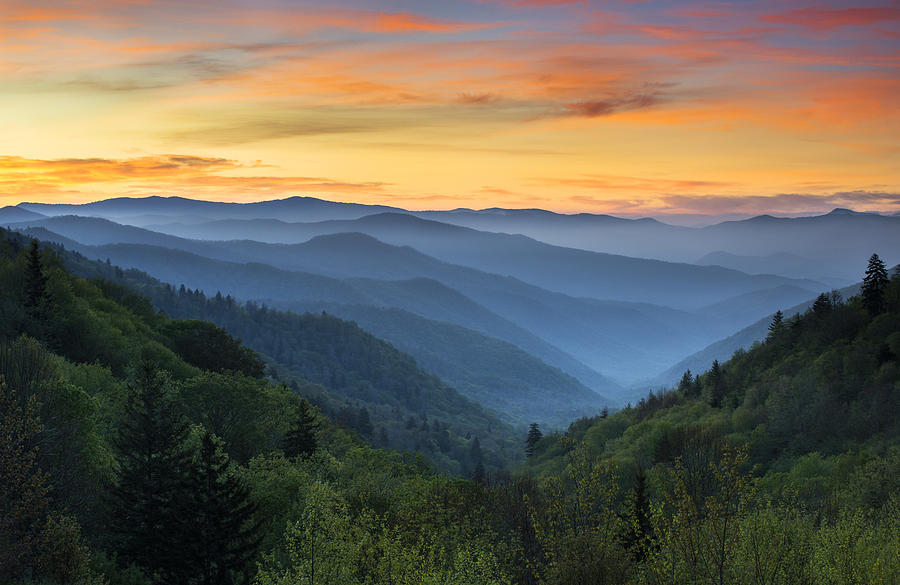
\includegraphics[width=\paperwidth,height =\paperheight]{Figures/smoky_mountains_sunrise_.jpg}}

% If you wish to uncover everything in a step-wise fashion, uncomment
% the following command: 

%\beamerdefaultoverlayspecification{<+->}
%%%%%%%%%%%%%%%%%%%%%%%%%%%%%%%%%%%%%%%%%%%%%%%%%%%%%%%%%%%%%%%%%%%%%%%%%%%%%%%%%%%
%%%%%%%%%%%%%%%%%%%%%%%%%%%%%%%%%%%%%%%%%%%%%%%%%%%%%%%%%%%%%%%%%%%%%%%%%%%%%%%%%%%
%%%%%%%%%%%%%%%%%%%%%%%%%%%%%%%%%%%%%%%%%%%%%%%%%%%%%%%%%%%%%%%%%%%%%%%%%%%%%%%%%%%
\begin{document}

\begin{frame}
  \titlepage
\end{frame}

\begin{frame}{Contents}
  \tableofcontents
  % You might wish to add the option [pausesections]
\end{frame}
%%%%%%%%%%%%%%%%%%%%%%%%%%%%%%%%%%%%%%%%%%%%%%%%%%%%%%%%%%%%%%%%%%%%%%%%%%%%%%%%%%%
%%%%%%%%%%%%%%%%%%%%%%%%%%%%%%%%%%%%%%%%%%%%%%%%%%%%%%%%%%%%%%%%%%%%%%%%%%%%%%%%%%%
\section{Introduction}
		
	\subsection{Great Smoky Mountains}
		\begin{frame}{Study area}

\begin{block}{Description of study area}
	\begin{itemize}
		\item Straddles the border of Tennessee and North Carolina
		\item Diverse wildlife, plant life, and fish life.
	\end{itemize}
\end{block}
 
\begin{figure}
\centering			
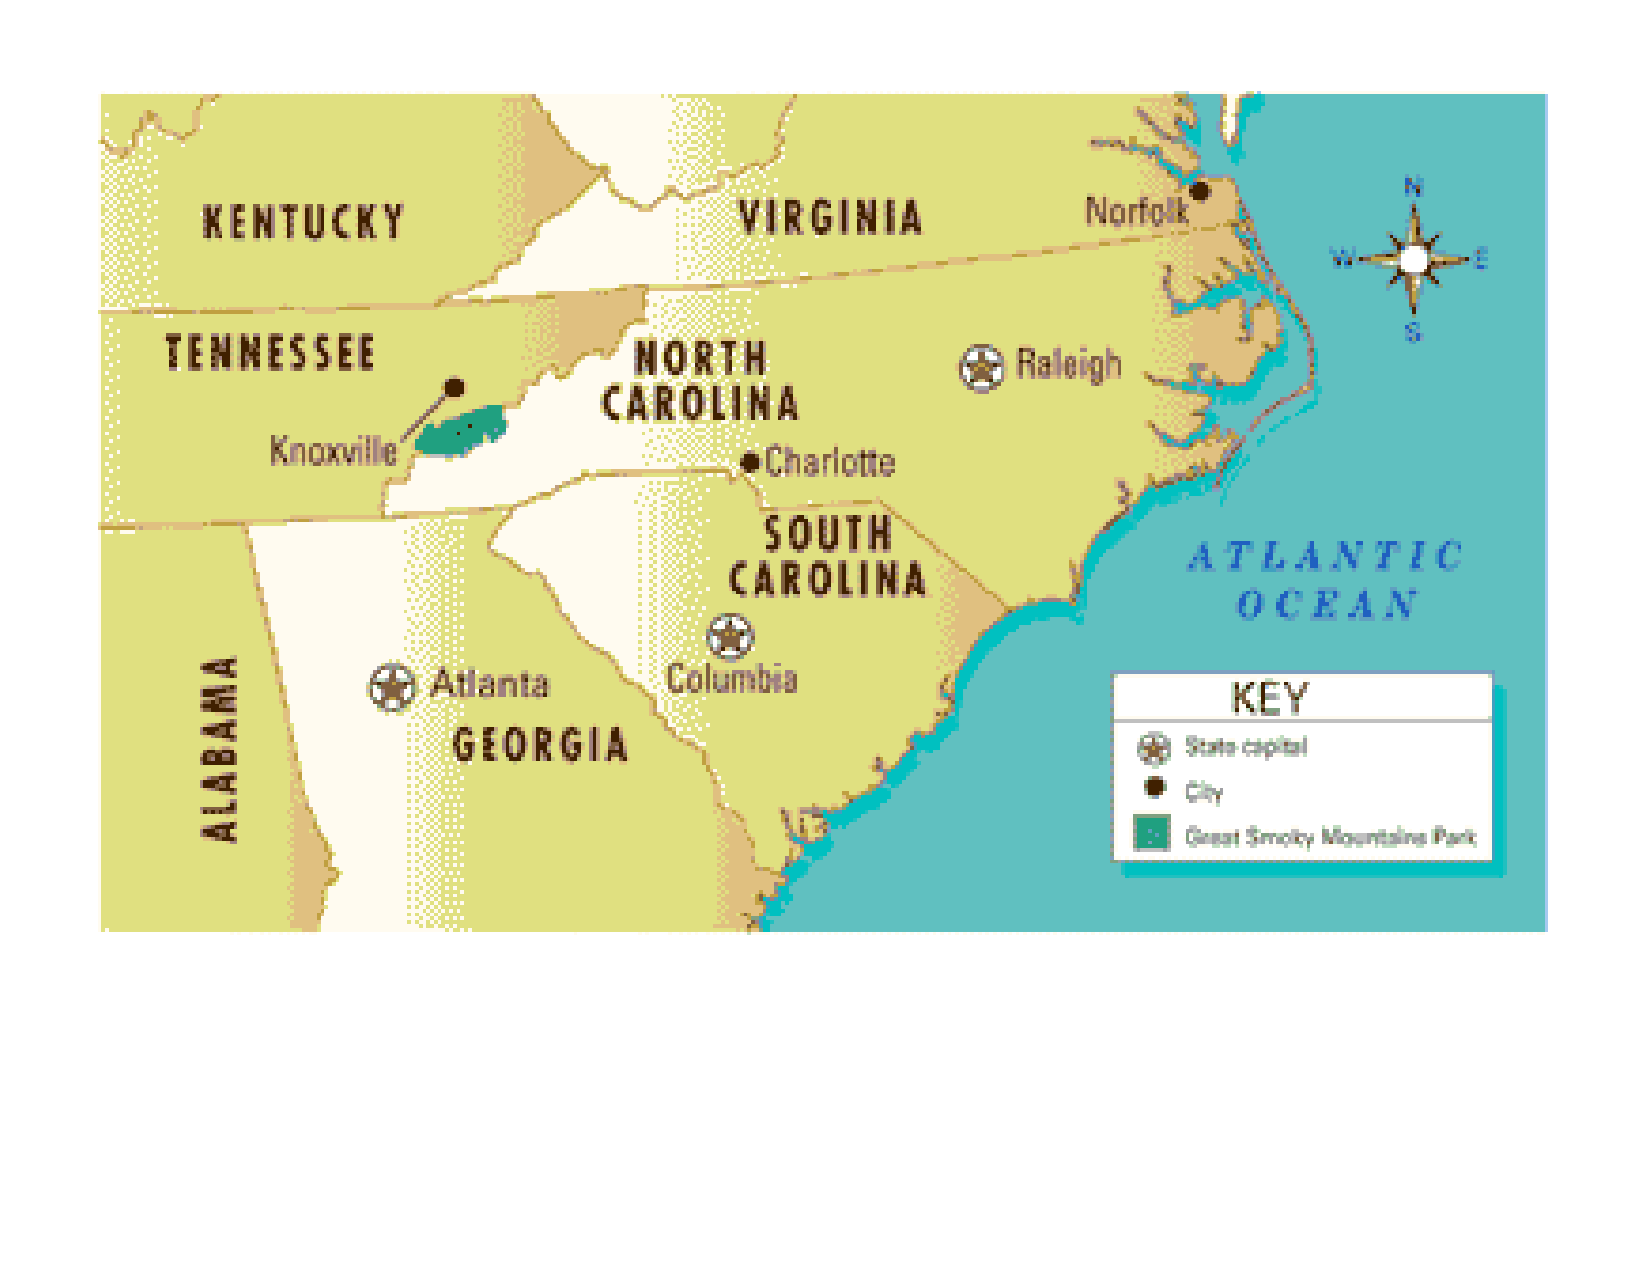
\includegraphics[width=.85\textwidth]{Figures/Parklocation2}
\end{figure}
		
\end{frame}

		\begin{frame}{Acid Deposition and the GRSM}

\begin{block}{Affects and effects}
	\begin{itemize}
		\item Acid deposition negatively affects the park.
		\item Higher elevations are effected worse.
	\end{itemize}
\end{block}
 
\begin{figure}
\centering			
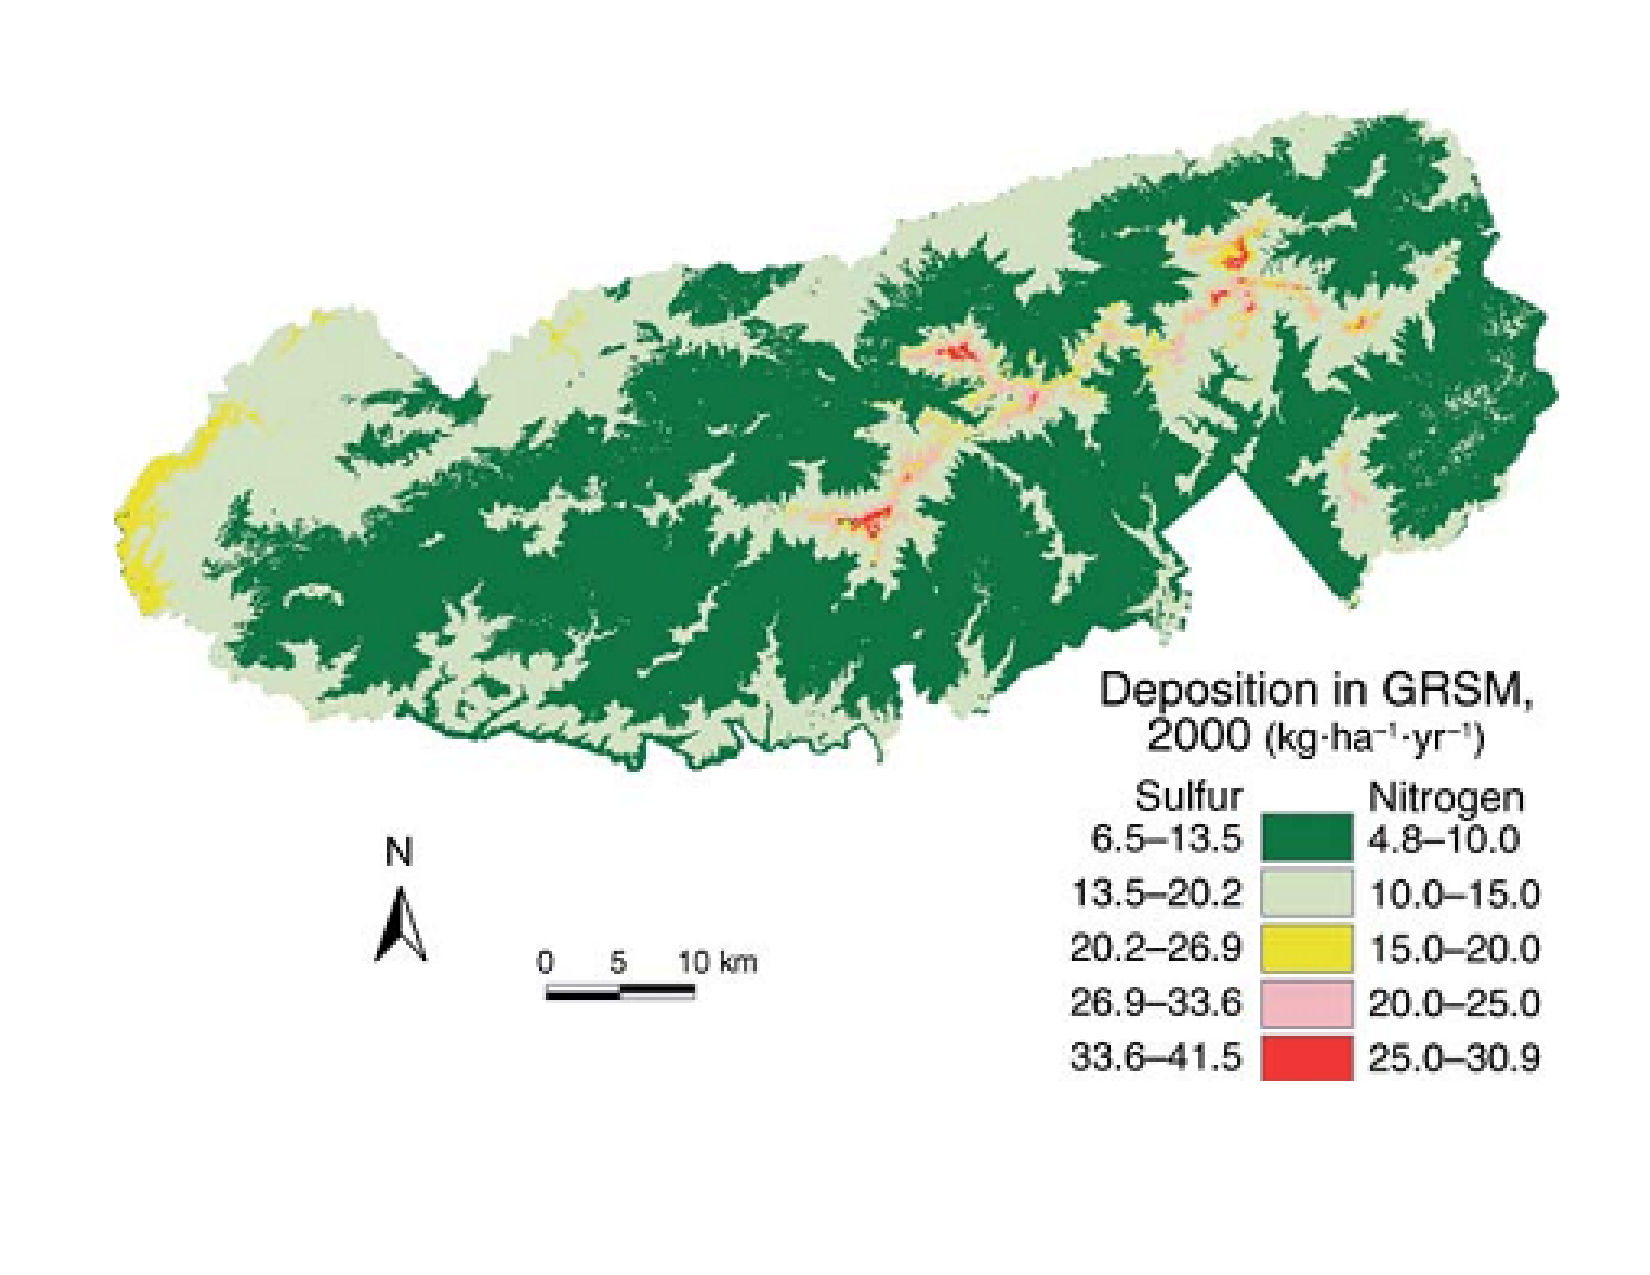
\includegraphics[width=.70\textwidth]{Figures/DepositionHeat}
\end{figure}
		
\end{frame}

	\subsection{Stream Survey}
		\begin{frame}{Database}

\begin{block}{Sites}
	\begin{itemize}
		\item 1993 - ongoing
		\item The number of sites monitored has decreased over the years
	\end{itemize}
\end{block}
 
\begin{figure}
\centering			
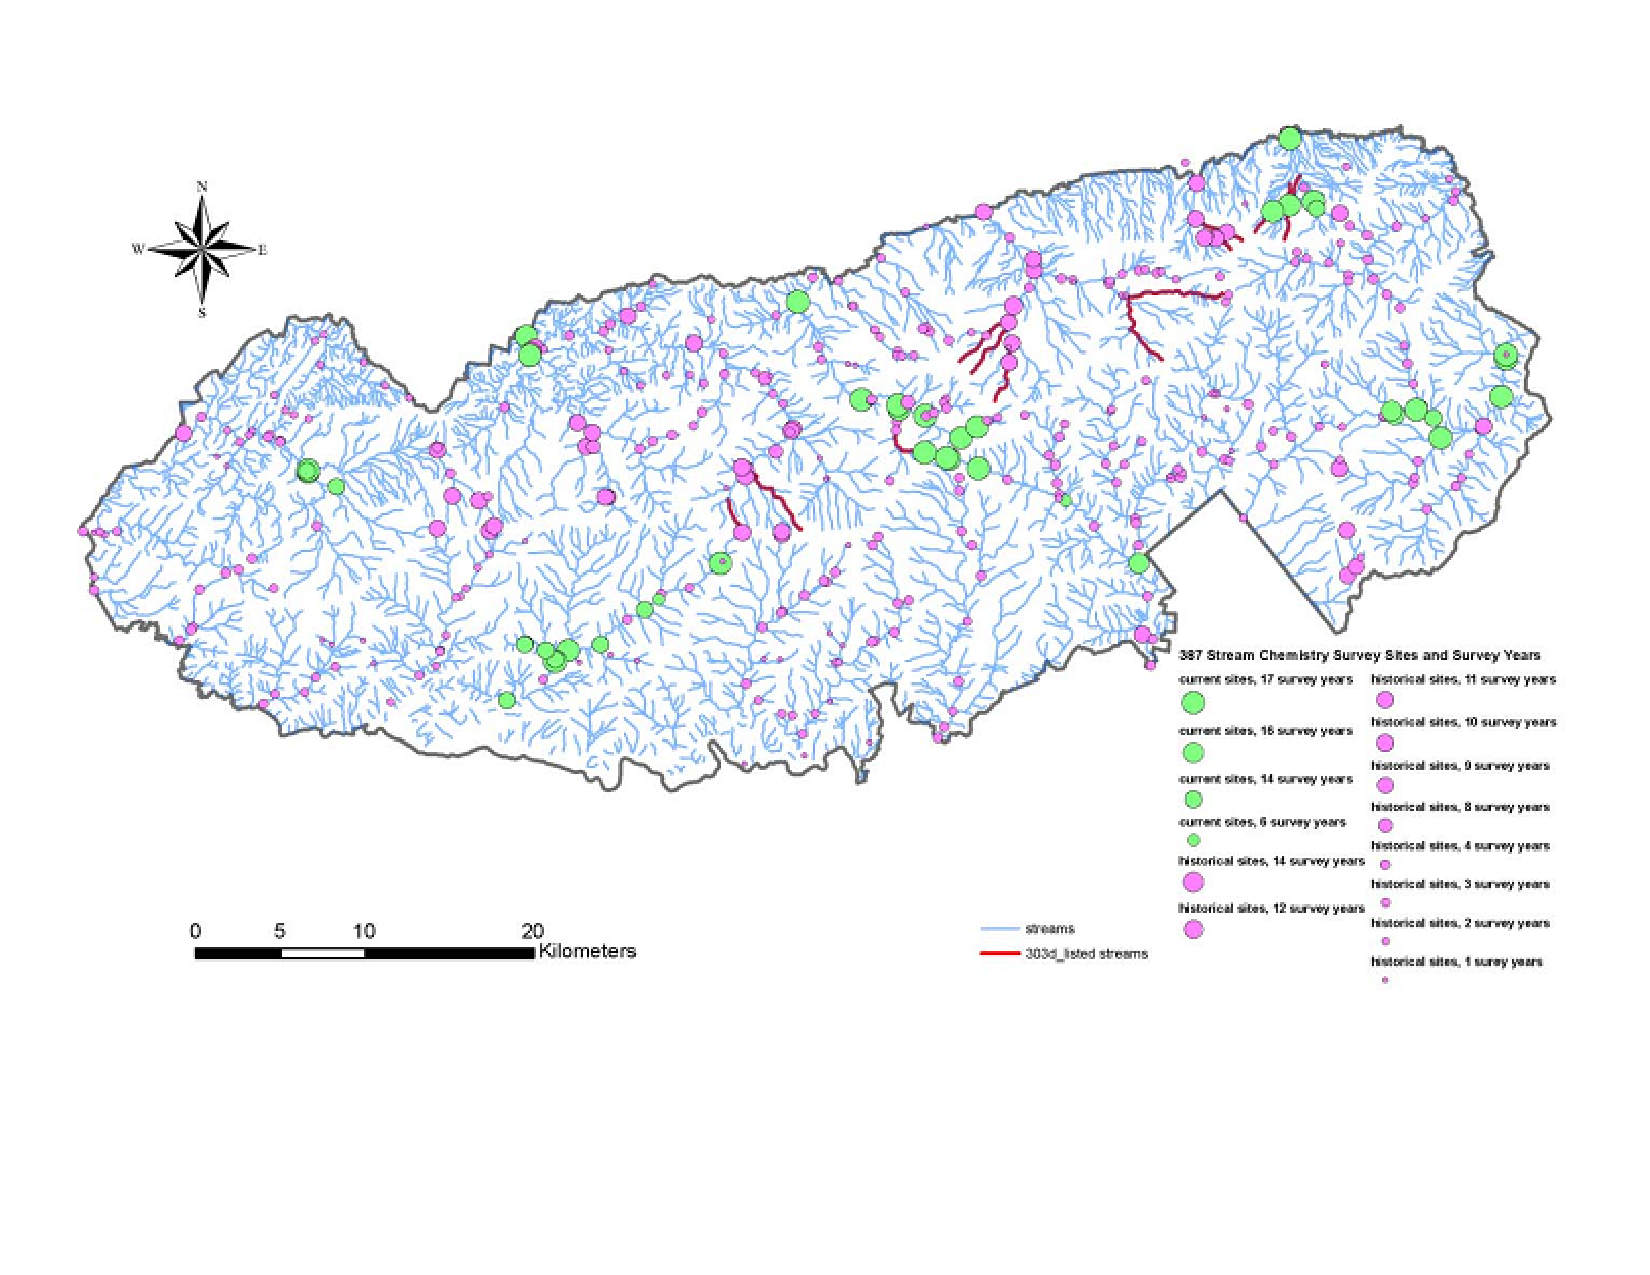
\includegraphics[width=.75\textwidth]{Figures/SSsites}
\end{figure}
		
\end{frame}

		\begin{frame}{Elevation Bands}

\begin{block}{Changes}
	\begin{itemize}
		\item 11 historical elevation bands
		\item re-organized into six	more powerful bands	
	\end{itemize}
\end{block}
			
\begin{table}[h]\footnotesize
%\caption[Proposed elevation classes]{These elevation classes were created to add more weight to the higher elevations.}
\begin{tabular}{p{1.5cm}p{2cm}cp{4.4cm}}
\toprule
Elevation Classes & Meters (Feet)                           & n & Site \# \\ 
\midrule

1                        & 304.8-609.6 (1000-2000)           & 5   & 13 ,23, 24, 30, 479 \\ 
2                        & 609.6-762 (2000-2500)              & 9   & 4, 311, 268, 480, 310, 483, 147, 148, 484 \\ 
3                        & 762-914.4 (2500-3000)              & 13 & 114, 481, 482, 149, 66, 492, 137, 293, 270, 493, 485, 144, 224 \\ 
4                        & 914.4-1066.8 (3000-3500)         & 4   & 143, 142, 73, 71 \\ 
5                        & 1066.8-1371.6 (3500-4500)       & 4   & 74, 221, 251, 233 \\ 
6                        & \multirow{2}{2cm}{$1371.6<$\\$(4500<)$}                    & 2   & 253, 234 \\ 
&&&\\
\bottomrule
\end{tabular}
%\label{tab:ElevationBands}
\end{table}
		
\end{frame}

		\begin{frame}{Time Sets}
	\begin{columns}
	\column{.5\textwidth}
	\begin{block}{3 separate sets}
		\begin{enumerate}
			\uncover<1>{\item \textcolor{blue}{1993-2002:} The years previously studied by Dr. Robinson}
			\uncover<2>{\item \textcolor{blue}{2003-2008:} Up to 2008, the year Kingston and Bull-run installed sulfate scrubbers}
			\uncover<3>{\item \textcolor{blue}{2009-2012:} After the scrubbers were installed up to the most recent data available}
		\end{enumerate}
	\end{block}
	
	\column{.5\textwidth}
	\only<1>{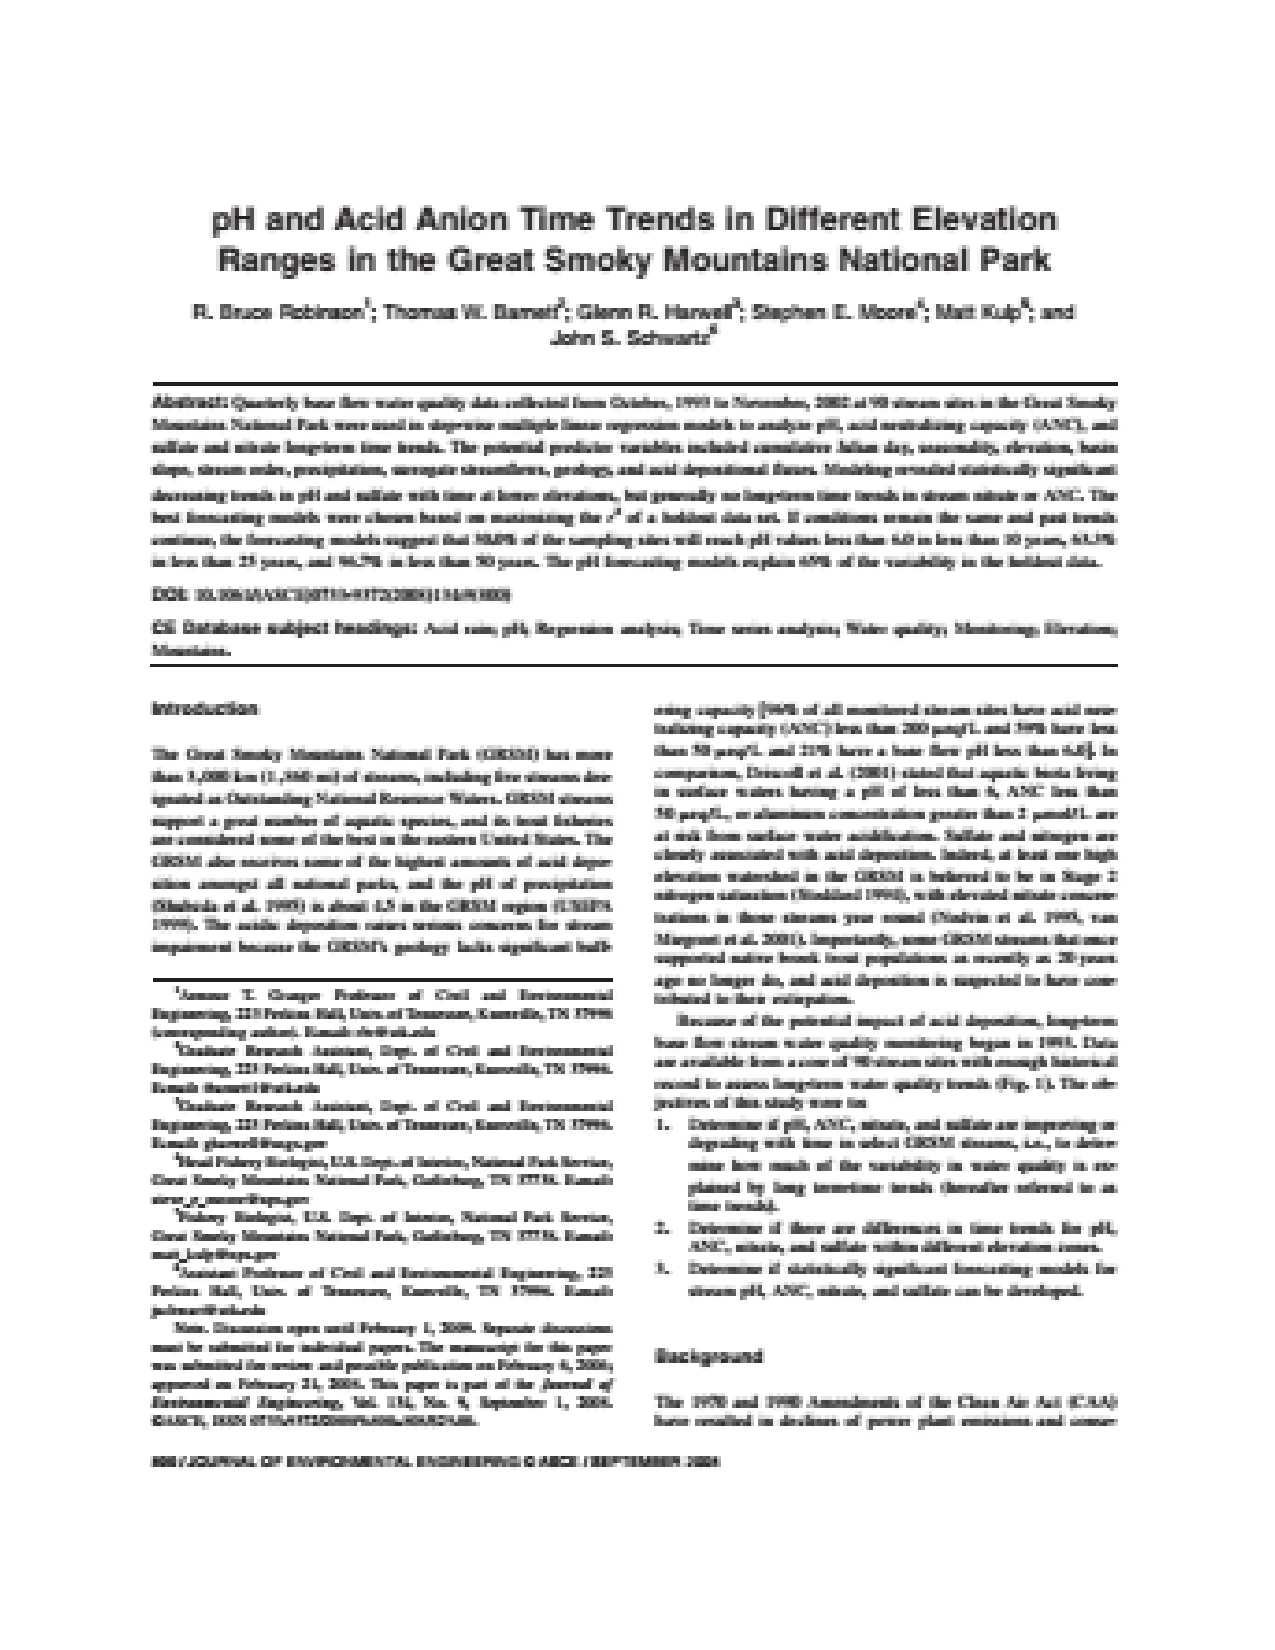
\includegraphics[width=\textwidth]{Figures/Robinson08}}
	\only<2>{\begin{figure}\centering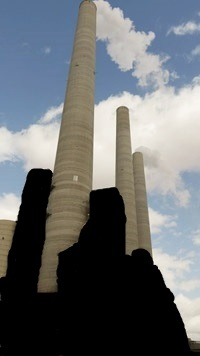
\includegraphics[width=.70\textwidth]{Figures/noscrubber.jpg}\end{figure}}
	\only<3>{\begin{figure}\centering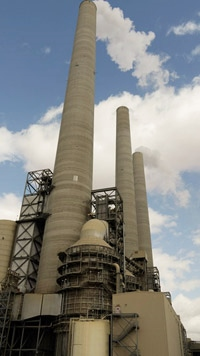
\includegraphics[width=.70\textwidth]{Figures/scrubber.jpg}\end{figure}}
	\end{columns}
\end{frame}
			
		\begin{frame}{Data Smoothing}

\begin{block}{Outliers and Influential observations}
	\begin{itemize}
		\item Influential observations are studied
			\begin{itemize}
				\item Removed Abrams and sites associated with Anakesta
				\item Others are reviewed individually
				\item Outliers remain
			\end{itemize}		
	\end{itemize}
\end{block}
 
\begin{figure}
\centering			
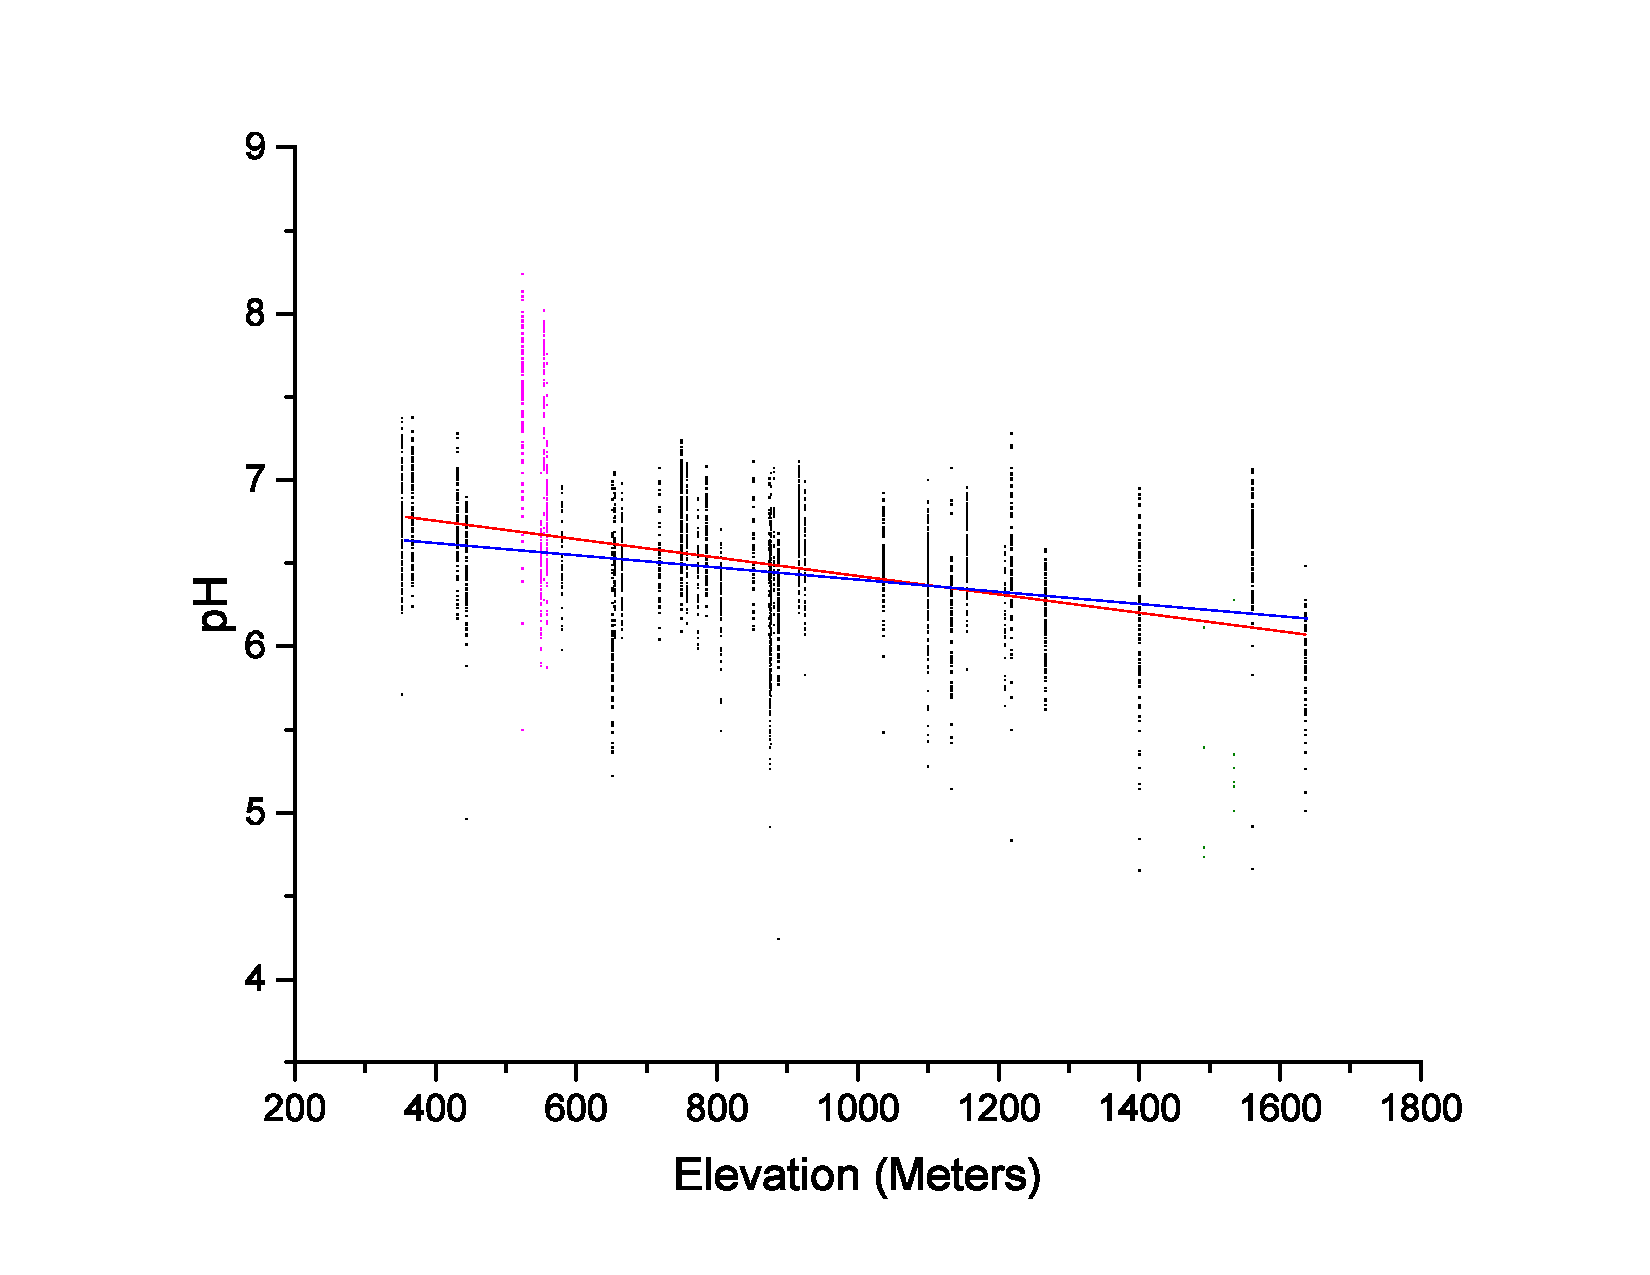
\includegraphics[width=.60\textwidth]{Figures/pHdata}
\end{figure}
		
\end{frame}

	\subsection{Objectives}
		\begin{frame}{Objectives}
	\begin{block}{One}
			 Determine conditions of stream pH and acidic anions within elevation bands.\pause
				\begin{itemize}
					\item Time trends
					\item Means Comparisons
				\end{itemize}\pause
	\end{block}
	\begin{block}{Two}
			Determine statistical power for water quality parameters.\pause
				\begin{itemize}
					\item Post Hoc Analysis
					\item A priori Analysis 
				\end{itemize}		
	\end{block}
\end{frame}

%%%%%%%%%%%%%%%%%%%%%%%%%%%%%%%%%%%%%%%%%%%%%%%%%%%%%%%%%%%%%%%%%%%%%%%%%%%%%%%%%%%
%%%%%%%%%%%%%%%%%%%%%%%%%%%%%%%%%%%%%%%%%%%%%%%%%%%%%%%%%%%%%%%%%%%%%%%%%%%%%%%%%%%
\section{Time Trend Analysis}

	\subsection{Regression}
		\begin{frame}{Stream Survey trend analysis history}
			\begin{columns}[T]
				\column{.5\textwidth}
					\begin{block}{Robinson 2008}%step-wise equations
						\begin{itemize}
						\uncover<1>{\item Time trends for water quality variables were computed for 90 sites in 10 elevation bands for the years 1993 to 2002.}
						\uncover<2>{\item Predictions for stream pH}
						\end{itemize}		
					\end{block}	
					\begin{block}{Biotics Effects report 2013}
						\begin{itemize}
							\uncover<3>{\item Time trends for water quality variables were computed for 67 sites for the years 1993 to 2009.}
						\end{itemize}		
					\end{block}	
				\column{.5\textwidth}
					\begin{block}{Results}				
						\only<1>{pH is \alert{decreasing} at at rate of -0.0127 to -0.0260 pH units/year for Elevation Classes 2-6.}
						\only<2>{pH will reach a deadly \alert{5.0} in 9.4 years in elevation class 6 (914-1067m)}
						\only<3>{\begin{itemize}
									\item Most showed no trend 
									\item 22 showed an \textcolor{blue}{increase} in pH 
								           \item Only 2 showed a \alert{decrease} 
							       \end{itemize}}
					\end{block}	
						\only<2>{\begin{figure}\centering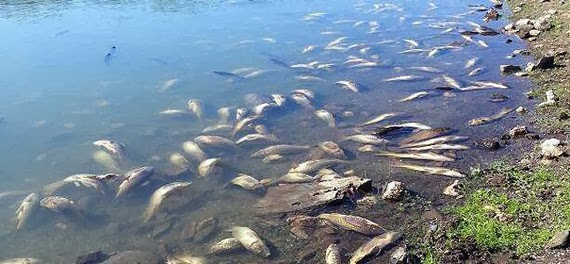
\includegraphics[width=\textwidth]{Figures/spaindeadfish.jpg}\end{figure}}
						\only<3>{\begin{figure}\centering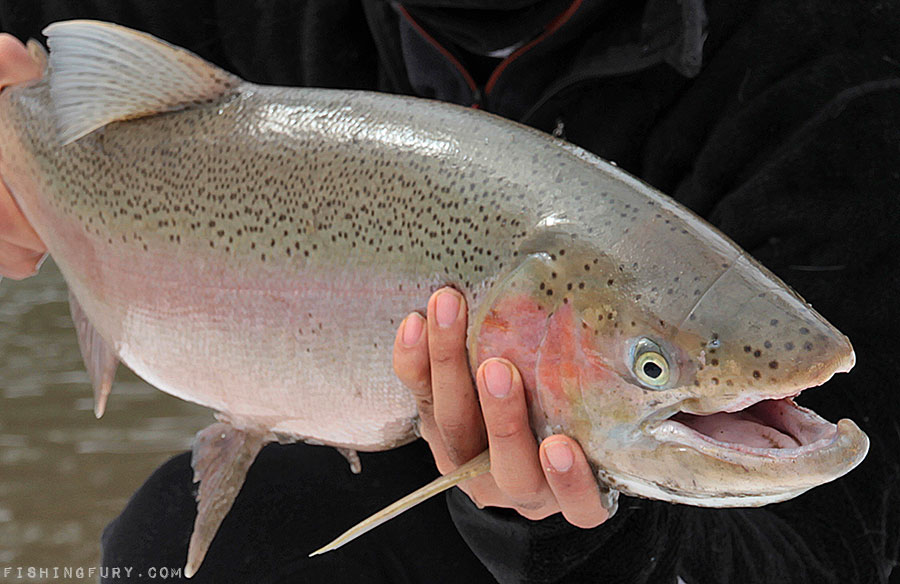
\includegraphics[width=.88\textwidth]{Figures/happy-trout1.jpg}\end{figure}}			
			\end{columns}
\end{frame}
	
		\begin{frame}<1-3>{Two equation methods}
	\only<1,3>{\begin{block}{Step-wise: $Y=\beta_0 + \beta_1  T + \beta_2  X + \beta_n X + \epsilon$}
		\begin{itemize}
			\item Multi-step process of adding and removing variables
			\item A variable with an F test statistic of .05 or higher can enter but would be removed if it exceeded .10. %goodness of fit test for the whole equation
			\item If any of the time variables were chosen by the step-wise method, the others were forced in.
		\end{itemize}
	\end{block}}

	\only<2>{\begin{table}[htbp]\scriptsize
\caption[Step-wise equations]{Equations created through step-wise variable selection}
\begin{tabular}{lp{5cm}cc}
\toprule
Dependent (n)     &Model                                                                                                                                                                                                                                                                                                                                                                                                       & Adjusted $r^2$  & Model p \\ 
\midrule
pH (3116)            &$.673\times\log_2(\text{Sum Base Cations}) + (-.368\times \text{NO}_3) + (.262\times \text{Julian Day}) + (-.266\times \text{SO}_4) + (-.050\times\cos(\theta))$                                                                                                                                       & 0.630                  & $<$0.001 \\
ANC (3116)         &$ (.415\times \text{Sum Base Cations}) + (-.185\times \text{SO}_4) + (.595\times \text{Conductivity}) + (-.102\times \text{NO}_3) + (.019\times \text{Julian Date}) + (.005\times \text{Cl}) + (.005\times \sin(\theta))$                                                & 0.984                  & 0.049 \\
NO$_3$ (3116)   &$(-.295\times \text{SO}_4) + (-3.183\times \text{ANC}) + (2.19\times \text{Conductivity}) + ( .923\times \text{Sum Base Cations}) + (.120\times \text{Julian Date}) + (.051\times \text{Cl}) + (.047\times \sin(\theta)) + (.031\times \cos(\theta))$ &0.498                   & 0.017 \\ 
SO$_4$ (3116)   &$ (-.166\times \text{NO}_3) + (2.318\times \text{Conductivity}) + (-3.229\times \text{ANC}) + (1.033\times \text{Sum Base Cations}) + (.042\times \text{Julian Date})$                                                                                                                               & 0.720                  & $<$0.001 \\ 
\bottomrule
\end{tabular}
\label{tab:stepwiseeq}
\end{table}
}

	\only<1,3>{\uncover<3>{\begin{block}{Time Variables: $Y= \beta_0 + \beta_1 Julian Date + \beta_2 \sin(\theta) + \beta_3 \cos(\theta) + \epsilon$}
		\begin{itemize}
			\item Remove the confusion caused by extra non-time based variables
			\item Inherently weaker because time doesn't explain all the variation of the dependent variables.
		\end{itemize}
	\end{block}}}
\end{frame}

	\subsection{Results}
		\begin{frame}{144 trends analyzed}
			\begin{columns}[T]
				\column{.35\textwidth}
					\begin{block}{Step-wise equations}
						\begin{itemize}[<+->]
							\item pH \uncover<2-8> {\textcolor{blue}{ increasing}}
							\item ANC \uncover<3-8> {\textcolor{blue}{ increasing}}
							\item Nitrate \uncover<4-8> {\alert{increasing}}
							\item Sulfate \uncover<5-8> {\textcolor{blue}{decreasing}}
						\end{itemize}
					\end{block}													
					\begin{block}{Time Variables}
							\uncover<5-8>{Only 20 of the 72 trends are significant}
						\begin{itemize}[<+->]
							\item pH \uncover<6-8> {\textcolor{blue}{ increasing}}
							\item ANC \uncover<7-8> {\textcolor{blue}{ increasing}}
							\item Nitrate
							\item Sulfate
						\end{itemize}
					\end{block}
				\column{.65\textwidth}
					\begin{block}{Trend Results}
						\only<1>{%pH
							      \begin{itemize}
							       	\item pH is \alert{negative} in only 3 significant lines, all in the 93'-02' time set, in elevation classes 2, 3, and 5
								\item Overall pH is \textcolor{blue}{ increasing} over time
							      \end{itemize}
							      }
						\only<2>{%ANC
							      \begin{itemize}
								\item Eleven \textcolor{blue}{positive} trends ranging from\\0.005 to 0.901 $\mu eq L^{-1}$
								\item Seven \alert{negative} trends ranging from\\ -0.002 to -0.082 $\mu eq L^{-1}$
								\item Overall ANC is \textcolor{blue}{ increasing} over time
							       \end{itemize}
							       }
						\only<3>{%Nitrate
							      \begin{itemize}
								\item Trends for time set 1 are half \alert{positive} and half \textcolor{blue}{negative}
								\item Trends in set 2 are all \alert{positive}, from 0.038 to 0.204 $\mu eq L^{-1}$
								\item There is only one \textcolor{blue}{decreasing} trend in set3, class 4 (-0.013 $\mu eq L^{-1}$)
								\item Overall nitrate is \alert{increasing} over time
							       \end{itemize}
							       }
						
						\only<4>{%Sulfate
							      \begin{itemize}
								\item All trends are \alert{positive} in set 2, ranging from 0.034 to 0.161 $\mu eq L^{-1}$
								\item Trends in set 3, classes 1, 3, and 6 are \textcolor{blue}{negative}
								\item Trends are \alert{increasing} from set 1 to set 2, \\ but \textcolor{blue}{decreasing} from set 2 to set 3
							       \end{itemize}
							       }
						\only<5>{%pH
							      \begin{itemize}
							       	\item Set 1 contains 0 significant lines and together sets 2 and 3 are half insignificant
								\item Other than prevalent insignificance, the trends for the time variables are similar to those of the the step-wise equations
								\item Overall pH is slowly \textcolor{blue}{ increasing} over time
							      \end{itemize}
							      }
						\only<6>{%ANC
							      \begin{itemize}
								\item Only 2 of the 24 trends are significant
								\item Set 1, class 5 has a \alert{decreasing} trend\\ of -0.148 $\mu eq L^{-1}$
								\item Set 3, class 5 has a \textcolor{blue}{increasing} trend\\ of 0.891 $\mu eq L^{-1}$
								\item Overall ANC is \textcolor{blue}{ increasing} over time
							      \end{itemize}
							     }
						\only<7>{%Nitrate
							      \begin{itemize}
								\item Only 6 of the 24 trends are significant, 2 in set 1, 4 in set 2, 0 in set 3
								\item Ever trend is \alert{increasing} except set 1, class 1, which is -0.138 $\mu eq L^{-1}$
								\item The increasing trends range from 0.155 $\mu eq/L$ to 0.330 $\mu eq L^{-1}$
								\item Overall nitrate is \alert{increasing} over time
								\item The trends are \textcolor{blue}{decreasing} from set 2 to 3, but all of set 3 is insignificant
							       \end{itemize}
							       }
						\only<8>{%Sulfate
							      \begin{itemize}
								\item Only 5 of the 24 trends are significant, 1 in set 1, 4 in set 2, 0 in set 3
								\item Ever trend is \alert{increasing} except set 1, class 1, which is -0.190 $\mu eq L^{-1}$
								\item The increasing trends range from 0.138 $\mu eq L^{-1}$ to 0.307 $\mu eq L^{-1}$
								\item Overall sulfate is \alert{increasing} over time 
								\item The trends are \textcolor{blue}{decreasing} from set 2 to 3, but all of set 3 is insignificant
							       \end{itemize}
							       }
					\end{block}
			\end{columns}
		\end{frame}
		
		\begin{frame}{Elevation trends}
	\begin{columns}
		\column{.35\textwidth}
			\begin{block}{Three Trends}			
				\begin{itemize}%[<+->]
					\uncover<1>{\item pH and ANC decrease as elevation increases}
					\uncover<2>{\item Nitrate, sulfate, and SBC all increase as elevation increases}
					\uncover<3>{\item Except for SBC all elevational trends decrease over time}
				\end{itemize}
			\end{block}
		\column{.65\textwidth}
			\only<1>{\begin{table}[htbp]\scriptsize
\centering
\caption[Elevation trends]{Dependents regressed against elevation.}
\begin{tabular}{llcccc}
\toprule
set & Dependent & n & slope&$r^2$&per +1000m \\ 
\midrule
1   & pH               & 1357 & .000 & .173 & \textcolor{cyan}{-0.411} \\ 
     & ANC            & 1354 & -.056 & .199 & \textcolor{cyan}{-56.227}  \\ 
     &  NO$_3^-$ & 1161 & .032 & .372 & 32.211  \\ 
     &  SO$_4^{2-}$& 1343 & .037 & .108 & 37.371  \\ 
     & SBC             & 1358 & .013 & .005 & 13.065 \\ 
\midrule
2   & pH               & 997 & .000 & .094 & \textcolor{cyan}{-0.391}  \\ 
     & ANC            & 997 & -.051 & .157 & \textcolor{cyan}{-50.970} \\ 
     &  NO$_3^-$  & 995 & .031 & .307 & 30.677  \\ 
     &  SO$_4^{2-}$ & 1029 & .036 & .098 & 35.793  \\ 
     & SBC             & 1031 & .016 & .009 & 15.537  \\ 
 \midrule
3   & pH              & 757 & .000 & .061 & \textcolor{cyan}{-0.286}  \\ 
     & ANC           & 757 & -.036 & .087 & \textcolor{cyan}{-35.689}  \\ 
     &  NO$_3^-$ & 757 & .026 & .195 & 25.924  \\ 
     &  SO$_4^{2-}$ & 757 & .030 & .101 & 29.715  \\ 
     & SBC            & 757 & .020 & .014 & 19.905  \\ 
 \bottomrule
\end{tabular}
\label{Water quality per elevation}
\end{table}
}
			\only<2>{\begin{table}[htbp]\scriptsize
\centering
\caption[Elevation trends]{Dependents regressed against elevation.}
\begin{tabular}{llcccc}
\toprule
set & Dependent & n & slope&$r^2$&per +1000m \\ 
\midrule
1   & pH               & 1357 & .000 & .173 & -0.411 \\ 
     & ANC            & 1354 & -.056 & .199 & -56.227  \\ 
     &  NO$_3^-$ & 1161 & .032 & .372 & \textcolor{cyan}{32.211}  \\ 
     &  SO$_4^{2-}$& 1343 & .037 & .108 & \textcolor{cyan}{37.371}  \\ 
     & SBC             & 1358 & .013 & .005 & \textcolor{cyan}{13.065} \\ 
\midrule
2   & pH               & 997 & .000 & .094 & -0.391  \\ 
     & ANC            & 997 & -.051 & .157 & -50.970 \\ 
     &  NO$_3^-$  & 995 & .031 & .307 & \textcolor{cyan}{30.677}  \\ 
     &  SO$_4^{2-}$ & 1029 & .036 & .098 & \textcolor{cyan}{35.793}  \\ 
     & SBC             & 1031 & .016 & .009 & \textcolor{cyan}{15.537} \\ 
 \midrule
3   & pH              & 757 & .000 & .061 & -0.286  \\ 
     & ANC           & 757 & -.036 & .087 & -35.689  \\ 
     &  NO$_3^-$ & 757 & .026 & .195 & \textcolor{cyan}{25.924}  \\ 
     &  SO$_4^{2-}$ & 757 & .030 & .101 & \textcolor{cyan}{29.715}  \\ 
     & SBC            & 757 & .020 & .014 & \textcolor{cyan}{19.905}  \\ 
 \bottomrule
\end{tabular}
\label{Water quality per elevation}
\end{table}
}
			\only<3>{\begin{table}[htbp]\scriptsize
\centering
\caption[Elevation trends]{Dependents regressed against elevation.}
\begin{tabular}{llcccc}
\toprule
set & Dependent & n & slope&$r^2$&per +1000m \\ 
\midrule
1   & pH               & 1357 & .000 & .173 & \textcolor{cyan}{-0.411} \\ 
     & ANC            & 1354 & -.056 & .199 & \textcolor{cyan}{-56.227}  \\ 
     &  NO$_3^-$ & 1161 & .032 & .372 & \textcolor{cyan}{32.211}  \\ 
     &  SO$_4^{2-}$& 1343 & .037 & .108 & \textcolor{cyan}{37.371}  \\ 
     & SBC             & 1358 & .013 & .005 & \textcolor{red}{13.065} \\ 
\midrule
2   & pH               & 997 & .000 & .094 & \textcolor{cyan}{-0.391}  \\ 
     & ANC            & 997 & -.051 & .157 & \textcolor{cyan}{-50.970} \\ 
     &  NO$_3^-$  & 995 & .031 & .307 & \textcolor{cyan}{30.677}  \\ 
     &  SO$_4^{2-}$ & 1029 & .036 & .098 & \textcolor{cyan}{35.793}  \\ 
     & SBC             & 1031 & .016 & .009 & \textcolor{red}{15.537}  \\ 
 \midrule
3   & pH              & 757 & .000 & .061 & \textcolor{cyan}{-0.286}  \\ 
     & ANC           & 757 & -.036 & .087 & \textcolor{cyan}{-35.689}  \\ 
     &  NO$_3^-$ & 757 & .026 & .195 & \textcolor{cyan}{25.924}  \\ 
     &  SO$_4^{2-}$ & 757 & .030 & .101 & \textcolor{cyan}{29.715}  \\ 
     & SBC            & 757 & .020 & .014 & \textcolor{red}{19.905}  \\ 
 \bottomrule
\end{tabular}
\label{Water quality per elevation}
\end{table}
}
		\end{columns}
\end{frame}	

		\begin{frame}{Elevation Trend Results by comparison}
	\begin{columns}[T]
		\column{.33\textwidth}
			\begin{block}{Robinson 08}
				\begin{itemize}
					\uncover<1>{\item pH decreases -0.72 pH units \\per 1000 m gain}
					\uncover<2>{\item Elevation not a predictor for any other dependent}
				\end{itemize}
			\end{block}
		\column{.33\textwidth}
			\begin{block}{Schwartz 13}
				\begin{itemize}
					\uncover<1>{\item pH decreases -1.056 pH units per 1000 m gain}
					\uncover<2>{\item ANC decreases -117.909 $\mu eq L^{-1}$ per 1000 m gain}
					\uncover<3>{\item Insignificant negative trend for sulfate}
				\end{itemize}
			\end{block}
		\column{.33\textwidth}
			\begin{block}{Pobst 14}
				\begin{itemize}
					\uncover<1>{\item pH decreases -0.0286 pH units per 1000 m gain}
					\uncover<2>{\item ANC decreases -35.689 $\mu eq L^{-1}$ per 1000 m gain}
					\uncover<3>{\item Positive sulfate elevational trends decrease over time}
					%\item SBC elevational trends increase over time\\ first by 2 $\mu eq L^{-1}$ between sets 1 and 2 \\ then by 5 $\mu eq L^{-1}$ between 2 and 3
				\end{itemize}
			\end{block}
	\end{columns}
\end{frame}	

		\begin{frame}{Data differences}
			\begin{columns}[T]
			\column{.33\textwidth}
				\begin{block}{Robinson 08}
					\begin{itemize}
						\item 90 sites
						\item 11 elevation classes		
						\item 1993 - 2002,\\ 10 years
						\item includes Abrams and sites 237 and 252
					\end{itemize}
				\end{block}
			\column{.33\textwidth}
				\begin{block}{Schwartz 13}
					\begin{itemize}
						\item 67 sites
						\item 11 elevation classes
						\item 1993 - 2009,\\ 17 years
					\end{itemize}
				\end{block}
			\column{.33\textwidth}
				\begin{block}{Pobst 14}
					\begin{itemize}
						\item 43 sites
						\item 6 elevation classes						
						\item set 1: 10 years
						\item set 2: 6 years
						\item set 3: 4 years
						\item removed Abrams and sites 237 and 252
					\end{itemize}
				\end{block}
			\end{columns}
		\end{frame}

	\subsection{Discussion and Conclusions}
		\begin{frame}{Conclusions}
	%\begin{block}{Copnclusions on elevation and time}
		%\begin{itemize}
			%\item elevation was not chosen through the step-wise process
			%\begin{itemize}	
				%\item elevation not as important as other variables
				%\item elevation classes already classify elevation
				%\item elevation classes may be to small for elevation to be important
			%\end{itemize}
			%\item Time may not explain enough variance to use regression for time trends
			%\item agree with the biotics effects report that pH is increasing over time
			%\item sulfate has more decreasing trends for set 3 than any other time set
		%\end{itemize}
	%\end{block}
	\only<1,3,5,6>{\begin{block}{Sulfate}
		Sulfate desorption is of greater concern than pH levels in the park
		\begin{itemize}
			%\item Lack of trend found in the Biotics effects report were attributed to high elevation soil adsorption of depsotional sulfate
				%sulfate pollution is held between deposition and the streams
			%\item Sulfate will remain absorbed to soil particles as long as soil water chemistry remains high in sulfate concentration and low in pH
				%when pH rises and sulfate concentration lowers the extra "held" sulfate pollution will make its way into the streams
			%\item sulfate elevation trends are decreasing overtime but mean concentrations are increasing through time
			\uncover<1-6>{\item Over time most sulfate trends are \alert{positive} but in set 3: classes 1, 4, and 6 have \textcolor{blue}{negative} trends (-0.052, -0.068, -0.059)}
			%\item Sulfate trends are all negative but insignificant in the time variable based trends
			\uncover<3-6>{\item The elevation trend is decreasing over the three time sets (37.371, 35.793, 29.715)}
			\uncover<5,6>{\item pH is \textcolor{blue}{increasing} while the sulfate trends are \textcolor{blue}{decreasing}}
			\uncover<6>{\item This combination could lead to sulfate desorption}
		\end{itemize}
	\end{block}}
\only<2>{% Table generated by Excel2LaTeX from sheet 'Julilan Date Coefficient'
\begin{table}\tiny
  \centering
  \caption{Julian date coefficients from step-wise regression for set 3.}
    \begin{tabular}{ccccccc}
    \toprule
    \multirow{3}[4]{1cm}{Elevation class} & \multirow{3}[4]{1cm}{Elevation range m (ft)} & \multirow{3}[4]{1cm}{Number of sites} & \multicolumn{4}{c}{\multirow{2}[2]{4cm}{Julian date coefficient, $\mu$eq/L or pH units (model adjusted r$^2$) (p-value)}} \\
          &       &       & \multicolumn{4}{c}{} \bigstrut\\\cline{4-7}\noalign{\smallskip}
          &       &       & pH    & ANC   & Nitrate & Sulfate \\
\midrule
    \multirow{3}[2]{*}{1} & \multirow{3}[2]{2.5cm}{304.8-609.6 (1000-2000)} & \multirow{3}[2]{*}{5} & 0.106  & -0.002  & 0.026  & \textcolor{blue}{-0.052}  \\
          &       &       & 0.894  & 0.989  & 0.376  & 0.536  \\
          &       &       & 0.000  & 0.000  & 0.000  & 0.000 \bigstrut\\\cline{4-7}\noalign{\smallskip}
    \multirow{3}[2]{*}{2} & \multirow{3}[2]{2.5cm}{609.6-762 (2000-2500)} & \multirow{3}[2]{*}{9} & 0.218  & 0.069  & 0.121  & 0.039  \\
          &       &       & 0.606  & 0.862  & 0.735  & 0.887  \\
          &       &       & 0.000  & 0.000  & 0.000  & 0.000 \bigstrut\\\cline{4-7}\noalign{\smallskip}
    \multirow{3}[2]{*}{3} & \multirow{3}[2]{2.5cm}{762-914.4 (2500-3000)} & \multirow{3}[2]{*}{13} & 0.056  & 0.007  & 0.019  & 0.050  \\
          &       &       & 0.766  & 0.997  & 0.598  & 0.915  \\
          &       &       & 0.000  & 0.000  & 0.000  & 0.000  \bigstrut\\\cline{4-7}\noalign{\smallskip}
    \multirow{3}[2]{*}{4} & \multirow{3}[2]{2.5cm}{914.4-1066.8 (3500-3500)} & \multirow{3}[2]{*}{4} & 0.413  & -0.006  & -0.013  & \textcolor{blue}{-0.068}  \\
          &       &       & 0.593  & 0.772  & 0.635  & 0.529  \\
          &       &       & 0.000  & 0.000  & 0.000  & 0.000  \bigstrut\\\cline{4-7}\noalign{\smallskip}
    \multirow{3}[2]{*}{5} & \multirow{3}[2]{2.5cm}{1066.8-1371.6 (3500-4500)} & \multirow{3}[2]{*}{4} & \textbf{-0.115 } & 0.901  & \textbf{0.098 } & 0.015  \\
          &       &       & \textbf{0.158 } & 0.540  & \textbf{-0.272 } & 0.658  \\
          &       &       & \textbf{0.130 } & 0.001  & \textbf{0.975 } & 0.000  \bigstrut\\\cline{4-7}\noalign{\smallskip}
    \multirow{3}[2]{*}{6} & \multirow{3}[2]{2.5cm}{1371.6$< (4500<$)} & \multirow{3}[2]{*}{2} & 0.289  & 0.059  & 0.097  & \textcolor{blue}{-0.059}  \\
          &       &       & 0.286  & 0.809  & 0.881  & 0.861  \\
          &       &       & 0.000  & 0.000  & 0.000  & 0.000  \\
    \bottomrule
    \end{tabular}%
  \label{tab:Set3SWJDl}%
\end{table}%
}
\only<4>{\begin{table}[htbp]\scriptsize
\centering
\caption[Elevation trends]{Dependents regressed against elevation.}
\begin{tabular}{llcccc}
\toprule
set & Dependent & n & slope&$r^2$&per +1000m \\ 
\midrule
1   & pH               & 1357 & .000 & .173 & -0.411  \\ 
     & ANC            & 1354 & -.056 & .199 & -56.227  \\ 
     &  NO$_3^-$ & 1161 & .032 & .372 & 32.211  \\ 
     &  SO$_4^{2-}$& 1343 & .037 & .108 & \textcolor{blue}{37.371}  \\ 
     & SBC             & 1358 & .013 & .005 & 13.065  \\ 
\midrule
2   & pH               & 997 & .000 & .094 & -0.391  \\ 
     & ANC            & 997 & -.051 & .157 & -50.970  \\ 
     &  NO$_3^-$  & 995 & .031 & .307 & 30.677  \\ 
     &  SO$_4^{2-}$ & 1029 & .036 & .098 & \textcolor{blue}{35.793}  \\ 
     & SBC             & 1031 & .016 & .009 & 15.537  \\ 
 \midrule
3   & pH              & 757 & .000 & .061 & -0.286  \\ 
     & ANC           & 757 & -.036 & .087 & -35.689  \\ 
     &  NO$_3^-$ & 757 & .026 & .195 & 25.924  \\ 
     &  SO$_4^{2-}$ & 757 & .030 & .101 & \textcolor{blue}{29.715}  \\ 
     & SBC            & 757 & .020 & .014 & 19.905  \\ 
 \bottomrule
\end{tabular}
\label{Water quality per elevation}
\end{table}
}
	
\end{frame}		
			
%%%%%%%%%%%%%%%%%%%%%%%%%%%%%%%%%%%%%%%%%%%%%%%%%%%%%%%%%%%%%%%%%%%%%%%%%%%%%%%%%%%
%%%%%%%%%%%%%%%%%%%%%%%%%%%%%%%%%%%%%%%%%%%%%%%%%%%%%%%%%%%%%%%%%%%%%%%%%%%%%%%%%%%
\section{ANOVA}
	
	\subsection{Introduction}
		\begin{frame}{Hypothesis}
			\only<1>{\begin{block}{}
				Is there a correlation between the decrease in Noland Divide TF sulfate concentrations and the decrease of sulfur dioxide emissions from Kingston and Bull run power plant emissions due to the installation of scrubbers in 2008?
			\end{block}}
			\only<2>{\begin{block}{}
				If there is a correlation between the decrease of sulfate concentrations and lowered sulfur dioxide emissions,\\ then time sets 2 and 3 will not be statistically equal.
					\end{block}}
			\begin{figure}\centering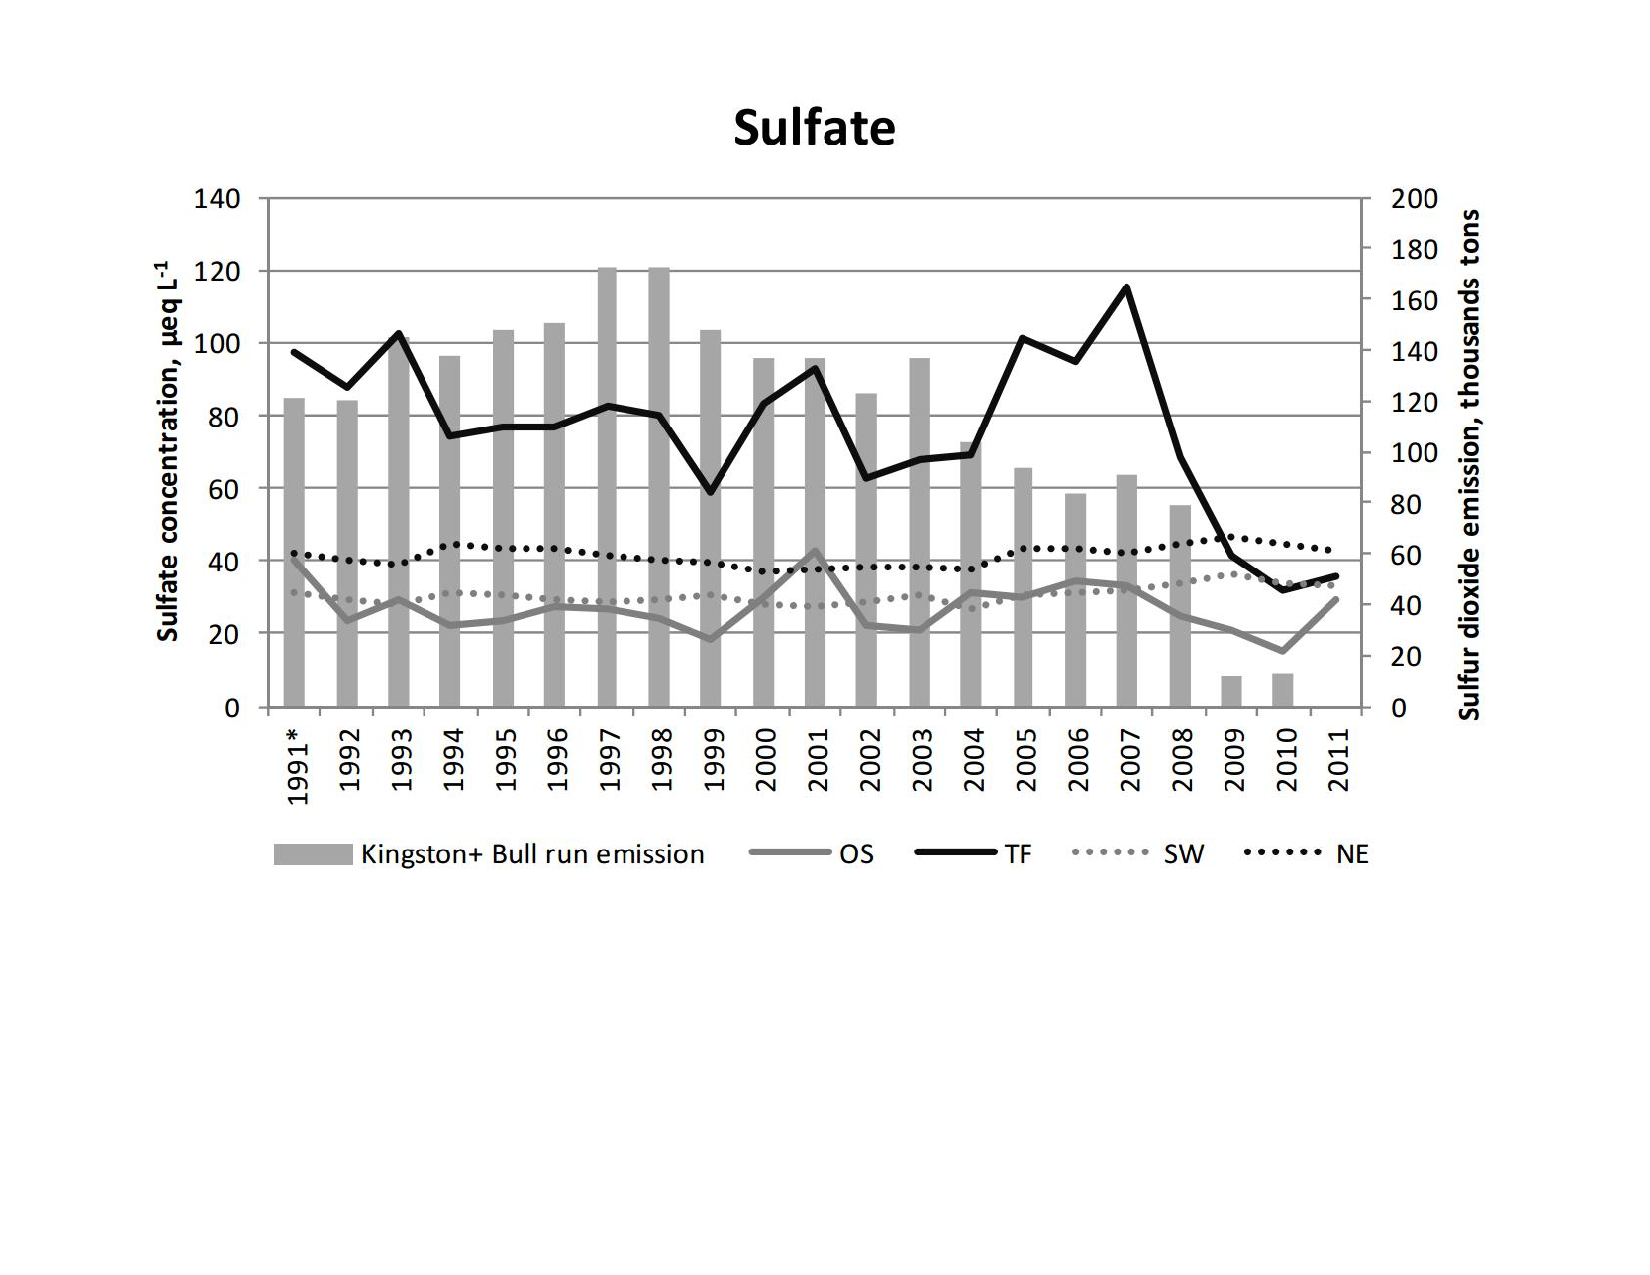
\includegraphics[width=.80\textwidth]{Figures/SulfateEmissions}\end{figure}
		\end{frame}%Interestingly the through fall SO4 concentrations dramatically decline from about 115 eq L in 2007 to about 30 in 2010

	\subsection{Methods}
		\begin{frame}{Method}	
		\begin{block}{Bonferroni}
				\begin{itemize}
					\item The three time sets will be tested against each other for sameness
					\item With more than 2 groups ANOVA cannot say which groups are the same or not the same
					\item The Bonferroni method can achieve this
					\begin{itemize}
						\item It will compare all time sets with each other in pairs (1:2, 1:3, 2:3)
						\item SPSS multiplies the p-value of the least significant differences (LSD) by the number of tests
						\item Insignificant comparisons are considered statistically equal
					\end{itemize}
				\end{itemize}
			\end{block}
			
		\end{frame}

	\subsection{Results}
			\begin{frame}{Group Comparisons}
			
					\only<1,2>{\begin{block}{pH}
						\begin{itemize}
							\uncover<1>{\item pH comparisons are more unequal than any other dependent}
							\uncover<2>{\item More inequalities versus set 3 than any other}		
						\end{itemize}
					\end{block}
						\only<1>{\begin{table}\scriptsize
%\caption{Bonferroni comparisons between multiple groups}
\begin{center}
\begin{tabular}{ccccccccccccc}
\toprule
 \multicolumn{1}{p{1cm}}{Elevation Classes}& \multicolumn{ 3}{c}{\textbf{pH}} & \multicolumn{ 3}{c}{ANC} & \multicolumn{ 3}{c}{Nitrate} & \multicolumn{ 3}{c}{Sulfate} \\ \cline{2-13}\noalign{\smallskip}
 & \multicolumn{ 1}{c}{\textbf{1-2}} & \textbf{1-3} & \textbf{2-3} & 1-2 & 1-3 &2-3 & 1-2 &1-3 &2-3&1-2 & 1-3 & 2-3 \\  \cline{2-13}
\multicolumn{1}{c}{1} & \textcolor{red}{\textbf{$\neq$}} & \textcolor{red}{\textbf{$\neq$}} & \textcolor{red}{\textbf{$\neq$}}                          & \textbf{=} & \textbf{=} & \textbf{=} & \textbf{$\neq$} & \textbf{=} & \textbf{=} & \textbf{=} & \textbf{=} & \textbf{=} \\ 
\multicolumn{1}{c}{2} & \textcolor{blue}{\textbf{=}} & \textcolor{blue}{\textbf{=}} & \textcolor{blue}{\textbf{=}}                                                & \textbf{=} & \textbf{$\neq$} & \textbf{=} & \textbf{$\neq$} & \textbf{$\neq$} & \textbf{=} & \textbf{$\neq$} & \textbf{$\neq$} & \textbf{=} \\ 
\multicolumn{1}{c}{3} & \textcolor{red}{\textbf{$\neq$}} & \textcolor{red}{\textbf{$\neq$}} & \textcolor{red}{\textbf{$\neq$}}                          & \textbf{=} & \textbf{$\neq$} & \textbf{=} & \textbf{=} & \textbf{$\neq$} & \textbf{$\neq$} & \textbf{=} & \textbf{=} & \textbf{=} \\ 
\multicolumn{1}{c}{4} & \textcolor{blue}{\textbf{=}} & \textcolor{red}{\textbf{$\neq$}} & \textcolor{red}{\textbf{$\neq$}}                                  & \textbf{=} & \textbf{=} & \textbf{=} & \textbf{=} & \textbf{=} & \textbf{=} & \textbf{=} & \textbf{=} & \textbf{=} \\ 
\multicolumn{1}{c}{5} & \textcolor{red}{\textbf{$\neq$}} & \textcolor{red}{\textbf{$\neq$}} & \textcolor{red}{\textbf{$\neq$}}                           & \textbf{=} & \textbf{$\neq$} & \textbf{$\neq$} & \textbf{$\neq$} & \textbf{=} & \textbf{$\neq$} & \textbf{=} & \textbf{=} & \textbf{=} \\ 
\multicolumn{1}{c}{6} & \textcolor{blue}{\textbf{=}} & \textcolor{red}{\textbf{$\neq$}} & \textcolor{red}{\textbf{$\neq$}}                                  & \textbf{=} & \textbf{=} & \textbf{=} & \textbf{=} & \textbf{=} & \textbf{=} & \textbf{=} & \textbf{=} & \textbf{=} \\ 
\bottomrule
\end{tabular}
\end{center}
%\label{tab:Bontable}
\end{table}}
						\only<2>{\begin{table}\scriptsize
%\caption{Bonferroni comparisons between multiple groups}
\begin{center}
\begin{tabular}{ccccccccccccc}
\toprule
\multicolumn{1}{p{1cm}}{Elevation Classes}& \multicolumn{ 3}{c}{pH}                                                                                            & \multicolumn{ 3}{c}{ANC}                                                                                             & \multicolumn{ 3}{c}{Nitrate}                                                                                                                           & \multicolumn{ 3}{c}{Sulfate}                                 \\ \cline{2-13}\noalign{\smallskip}
                                                                       & \multicolumn{ 1}{c}{\textcolor{gray}{1-2}} & \textbf{1-3}    &\textbf{2-3}          & \textcolor{gray}{1-2}                                    & \textbf{1-3}     & \textbf{2-3}          & \textcolor{gray}{1-2}                                           & \textbf{1-3}                      & \textbf{2-3}                     & \textcolor{gray}{1-2}                       & \textbf{1-3}                     & \textbf{2-3}             \\  \cline{2-13}
\multicolumn{1}{c}{1}                                    & \textcolor{gray}{\textbf{$\neq$}}               & \textcolor{red}{\textbf{$\neq$}}             & \textcolor{red}{\textbf{$\neq$}}                  & \textcolor{gray}{\textbf{=}}                        & \textcolor{blue}{\textbf{=}}                         & \textcolor{blue}{\textbf{=}}                              & \textcolor{gray}{\textbf{$\neq$}}                      & \textcolor{blue}{\textbf{=}}           & \textcolor{blue}{\textbf{=}}           & \textcolor{gray}{\textbf{=}}          & \textcolor{blue}{\textbf{=}}         & \textcolor{blue}{\textbf{=}}  \\ 
\multicolumn{1}{c}{2}                                    & \textcolor{gray}{\textbf{=}}                        & \textcolor{blue}{\textbf{=}}                     & \textcolor{blue}{\textbf{=}}                            & \textcolor{gray}{\textbf{=}}                        & \textcolor{red}{\textbf{$\neq$}}             & \textcolor{blue}{\textbf{=}}                               & \textcolor{gray}{\textbf{$\neq$}}                      & \textcolor{red}{\textbf{$\neq$}} & \textcolor{blue}{\textbf{=}}           & \textcolor{gray}{\textbf{$\neq$}} & \textcolor{red}{\textbf{$\neq$}}  & \textcolor{blue}{\textbf{=}}  \\ 
\multicolumn{1}{c}{3}                                    & \textcolor{gray}{\textbf{$\neq$}}               & \textcolor{red}{\textbf{$\neq$}}             & \textcolor{red}{\textbf{$\neq$}}                & \textcolor{gray}{\textbf{=}}                        & \textcolor{red}{\textbf{$\neq$}}             & \textcolor{blue}{\textbf{=}}                               & \textcolor{gray}{\textbf{=}}                               & \textcolor{red}{\textbf{$\neq$}} & \textcolor{red}{\textbf{$\neq$}} & \textcolor{gray}{\textbf{=}}          & \textcolor{blue}{\textbf{=}}         & \textcolor{blue}{\textbf{=}}  \\ 
\multicolumn{1}{c}{4}                                    & \textcolor{gray}{\textbf{=}}                        &\textcolor{red}{\textbf{$\neq$}}              & \textcolor{red}{\textbf{$\neq$}}                   & \textcolor{gray}{\textbf{=}}                        & \textcolor{blue}{\textbf{=}}                         & \textcolor{blue}{\textbf{=}}                               & \textcolor{gray}{\textbf{=}}                                & \textcolor{blue}{\textbf{=}}          & \textcolor{blue}{\textbf{=}}           & \textcolor{gray}{\textbf{=}}          & \textcolor{blue}{\textbf{=}}        & \textcolor{blue}{\textbf{=}} \\ 
\multicolumn{1}{c}{5}                                    & \textcolor{gray}{\textbf{$\neq$}}               & \textcolor{red}{\textbf{$\neq$}}             & \textcolor{red}{\textbf{$\neq$}}                & \textcolor{gray}{\textbf{=}}                        & \textcolor{red}{\textbf{$\neq$}}             & \textcolor{red}{\textbf{$\neq$}}                   & \textcolor{gray}{\textbf{$\neq$}}                       & \textcolor{blue}{\textbf{=}}           & \textcolor{red}{\textbf{$\neq$}} & \textcolor{gray}{\textbf{=}}          & \textcolor{blue}{\textbf{=}}         & \textcolor{blue}{\textbf{=}}  \\ 
\multicolumn{1}{c}{6}                                    & \textcolor{gray}{\textbf{=}}                        & \textcolor{red}{\textbf{$\neq$}}            & \textcolor{red}{\textbf{$\neq$}}                   & \textcolor{gray}{\textbf{=}}                        & \textcolor{blue}{\textbf{=}}                         & \textcolor{blue}{\textbf{=}}                               & \textcolor{gray}{\textbf{=}}                                & \textcolor{blue}{\textbf{=}}           & \textcolor{blue}{\textbf{=}}          & \textcolor{gray}{\textbf{=}}          & \textcolor{blue}{\textbf{=}}         & \textcolor{blue}{\textbf{=}} \\  
\bottomrule
\end{tabular}
\end{center}
%\label{tab:Bontable}
\end{table}}
							}
					\only<3,4>{\begin{block}{ANC}
						\begin{itemize}		
							\uncover<3>{\item More equal than unequal groups}
							\uncover<4>{\item Sets 1 and 2 are always equal, not so with set 3} 				
						\end{itemize}
					\end{block}
						\only<3,4>{\begin{table}\scriptsize
%\caption{Bonferroni comparisons between multiple groups}
\begin{center}
\begin{tabular}{ccccccccccccc}
\toprule
\multicolumn{1}{p{1cm}}{Elevation Classes}& \multicolumn{ 3}{c}{\textcolor{gray}{pH}}                                                                & \multicolumn{ 3}{c}{\textbf{ANC}}                                         & \multicolumn{ 3}{c}{\textcolor{gray}{Nitrate}}                                         & \multicolumn{ 3}{c}{\textcolor{gray}{Sulfate}}                                 \\ \cline{2-13}\noalign{\smallskip}
                                                                       & \multicolumn{ 1}{c}{\textcolor{gray}{1-2}} & \textcolor{gray}{1-3}                       & \textcolor{gray}{2-3}                      & \textbf{1-2}             & \textbf{1-3}                        & \textbf{2-3}                      & \textcolor{gray}{1-2}                     & \textcolor{gray}{1-3}                      & \textcolor{gray}{2-3}                     & \textcolor{gray}{1-2}                       & \textcolor{gray}{1-3}                     & \textcolor{gray}{2-3}             \\  \cline{2-13}
\multicolumn{1}{c}{1}                                    & \textcolor{gray}{\textbf{$\neq$}}               & \textcolor{gray}{\textbf{$\neq$}}  & \textcolor{gray}{\textbf{$\neq$}} & \textcolor{blue}{\textbf{=}} & \textcolor{blue}{\textbf{=}}           & \textcolor{blue}{\textbf{=}}          & \textcolor{gray}{\textbf{$\neq$}} & \textcolor{gray}{\textbf{=}}         & \textcolor{gray}{\textbf{=}}          & \textcolor{gray}{\textbf{=}}          & \textcolor{gray}{\textbf{=}}         & \textcolor{gray}{\textbf{=}} \\ 
\multicolumn{1}{c}{2}                                    & \textcolor{gray}{\textbf{=}}                        & \textcolor{gray}{\textbf{=}}          & \textcolor{gray}{\textbf{=}}          & \textcolor{blue}{\textbf{=}} & \textcolor{red}{\textbf{$\neq$}}    & \textcolor{blue}{\textbf{=}}          & \textcolor{gray}{\textbf{$\neq$}} & \textcolor{gray}{\textbf{$\neq$}} & \textcolor{gray}{\textbf{=}}          & \textcolor{gray}{\textbf{$\neq$}} & \textcolor{gray}{\textbf{$\neq$}} & \textcolor{gray}{\textbf{=}} \\ 
\multicolumn{1}{c}{3}                                    & \textcolor{gray}{\textbf{$\neq$}}               & \textcolor{gray}{\textbf{$\neq$}}  & \textcolor{gray}{\textbf{$\neq$}} & \textcolor{blue}{\textbf{=}} & \textcolor{red}{\textbf{$\neq$}}    & \textcolor{blue}{\textbf{=}}          & \textcolor{gray}{\textbf{=}}          & \textcolor{gray}{\textbf{$\neq$}} & \textcolor{gray}{\textbf{$\neq$}} & \textcolor{gray}{\textbf{=}}          & \textcolor{gray}{\textbf{=}}         &\textcolor{gray}{\textbf{=}} \\ 
\multicolumn{1}{c}{4}                                    & \textcolor{gray}{\textbf{=}}                        & \textcolor{gray}{\textbf{$\neq$}}  & \textcolor{gray}{\textbf{$\neq$}} & \textcolor{blue}{\textbf{=}} & \textcolor{blue}{\textbf{=}}             & \textcolor{blue}{\textbf{=}}          & \textcolor{gray}{\textbf{=}}          &\textcolor{gray}{\textbf{=}}         & \textcolor{gray}{\textbf{=}}          & \textcolor{gray}{\textbf{=}}          & \textcolor{gray}{\textbf{=}}         & \textcolor{gray}{\textbf{=}} \\ 
\multicolumn{1}{c}{5}                                    & \textcolor{gray}{\textbf{$\neq$}}               & \textcolor{gray}{\textbf{$\neq$}}  & \textcolor{gray}{\textbf{$\neq$}}  & \textcolor{blue}{\textbf{=}} & \textcolor{red}{\textbf{$\neq$}}    & \textcolor{red}{\textbf{$\neq$}} & \textcolor{gray}{\textbf{$\neq$}} & \textcolor{gray}{\textbf{=}}          & \textcolor{gray}{\textbf{$\neq$}} & \textcolor{gray}{\textbf{=}}          & \textcolor{gray}{\textbf{=}}         & \textcolor{gray}{\textbf{=}} \\ 
\multicolumn{1}{c}{6}                                    & \textcolor{gray}{\textbf{=}}                        & \textcolor{gray}{\textbf{$\neq$}}  & \textcolor{gray}{\textbf{$\neq$}}  & \textcolor{blue}{\textbf{=}}& \textcolor{blue}{\textbf{=}}            & \textcolor{blue}{\textbf{=}}          & \textcolor{gray}{\textbf{=}}          & \textcolor{gray}{\textbf{=}}          & \textcolor{gray}{\textbf{=}}         & \textcolor{gray}{\textbf{=}}          & \textcolor{gray}{\textbf{=}}         & \textcolor{gray}{\textbf{=}} \\ 
\bottomrule
\end{tabular}
\end{center}
%\label{tab:Bontable}
\end{table}
}
							}
					\only<5,6>{\begin{block}{Nitrate}
						\begin{itemize}
							\uncover<5>{\item Classes 4 and 6 are equal across all time sets}
							\uncover<6>{\item Difference in means seems to move up in elevation}	
						\end{itemize}
					\end{block}
						\only<5,6>{\begin{table}\scriptsize
%\caption{Bonferroni comparisons between multiple groups}
\begin{center}
\begin{tabular}{ccccccccccccc}
\toprule
\multicolumn{1}{p{1cm}}{Elevation Classes}& \multicolumn{ 3}{c}{\textcolor{gray}{pH}}                                                                & \multicolumn{ 3}{c}{\textcolor{gray}{ANC}}                                         & \multicolumn{ 3}{c}{\textbf{Nitrate}}                                         & \multicolumn{ 3}{c}{\textcolor{gray}{Sulfate}}                                 \\ \cline{2-13}\noalign{\smallskip}
                                                                       & \multicolumn{ 1}{c}{\textcolor{gray}{1-2}} & \textcolor{gray}{1-3}                       & \textcolor{gray}{2-3}                      & \textcolor{gray}{1-2}             & \textcolor{gray}{1-3}                        & \textcolor{gray}{2-3}                      & \textbf{1-2}                     & \textbf{1-3}                      & \textbf{2-3}                     & \textcolor{gray}{1-2}                       & \textcolor{gray}{1-3}                     & \textcolor{gray}{2-3}             \\  \cline{2-13}
\multicolumn{1}{c}{1}                                    & \textcolor{gray}{\textbf{$\neq$}}               & \textcolor{gray}{\textbf{$\neq$}}  & \textcolor{gray}{\textbf{$\neq$}} & \textcolor{gray}{\textbf{=}} & \textcolor{gray}{\textbf{=}}            & \textcolor{gray}{\textbf{=}}          & \textcolor{red}{\textbf{$\neq$}} & \textcolor{blue}{\textbf{=}}          & \textcolor{blue}{\textbf{=}}           & \textcolor{gray}{\textbf{=}}          & \textcolor{gray}{\textbf{=}}         & \textcolor{gray}{\textbf{=}} \\ 
\multicolumn{1}{c}{2}                                    & \textcolor{gray}{\textbf{=}}                        & \textcolor{gray}{\textbf{=}}          & \textcolor{gray}{\textbf{=}}          & \textcolor{gray}{\textbf{=}} & \textcolor{gray}{\textbf{$\neq$}}    & \textcolor{gray}{\textbf{=}}          & \textcolor{red}{\textbf{$\neq$}} & \textcolor{red}{\textbf{$\neq$}} & \textcolor{blue}{\textbf{=}}           & \textcolor{gray}{\textbf{$\neq$}} & \textcolor{gray}{\textbf{$\neq$}} & \textcolor{gray}{\textbf{=}} \\ 
\multicolumn{1}{c}{3}                                    &\textcolor{gray}{\textbf{$\neq$}}               & \textcolor{gray}{\textbf{$\neq$}}  & \textcolor{gray}{\textbf{$\neq$}} & \textcolor{gray}{\textbf{=}} & \textcolor{gray}{\textbf{$\neq$}}    & \textcolor{gray}{\textbf{=}}          & \textcolor{blue}{\textbf{=}}          & \textcolor{red}{\textbf{$\neq$}} & \textcolor{red}{\textbf{$\neq$}} & \textcolor{gray}{\textbf{=}}          & \textcolor{gray}{\textbf{=}}         & \textcolor{gray}{\textbf{=}} \\ 
\multicolumn{1}{c}{4}                                    & \textcolor{gray}{\textbf{=}}                        & \textcolor{gray}{\textbf{$\neq$}}  & \textcolor{gray}{\textbf{$\neq$}} & \textcolor{gray}{\textbf{=}} & \textcolor{gray}{\textbf{=}}             & \textcolor{gray}{\textbf{=}}          &\textcolor{blue}{\textbf{=}}          & \textcolor{blue}{\textbf{=}}          & \textcolor{blue}{\textbf{=}}           & \textcolor{gray}{\textbf{=}}          & \textcolor{gray}{\textbf{=}}         & \textcolor{gray}{\textbf{=}} \\ 
\multicolumn{1}{c}{5}                                    & \textcolor{gray}{\textbf{$\neq$}}               & \textcolor{gray}{\textbf{$\neq$}}  & \textcolor{gray}{\textbf{$\neq$}}  & \textcolor{gray}{\textbf{=}} & \textcolor{gray}{\textbf{$\neq$}}    & \textcolor{gray}{\textbf{$\neq$}} & \textcolor{red}{\textbf{$\neq$}} & \textcolor{blue}{\textbf{=}}           & \textcolor{red}{\textbf{$\neq$}} & \textcolor{gray}{\textbf{=}}          & \textcolor{gray}{\textbf{=}}         & \textcolor{gray}{\textbf{=}} \\ 
\multicolumn{1}{c}{6}                                    & \textcolor{gray}{\textbf{=}}                        & \textcolor{gray}{\textbf{$\neq$}}  & \textcolor{gray}{\textbf{$\neq$}}  & \textcolor{gray}{\textbf{=}} & \textcolor{gray}{\textbf{=}}            & \textcolor{gray}{\textbf{=}}          & \textcolor{blue}{\textbf{=}}           & \textcolor{blue}{\textbf{=}}           & \textcolor{blue}{\textbf{=}}         & \textcolor{gray}{\textbf{=}}          & \textcolor{gray}{\textbf{=}}         & \textcolor{gray}{\textbf{=}} \\ 
\bottomrule
\end{tabular}
\end{center}
%\label{tab:Bontable}
\end{table}}
							}
					\only<7,8>{\begin{block}{Sulfate}
						\begin{itemize}
							\uncover<7>{\item All sets are equal for all classes except for comparisons in class 2}
							\uncover<8>{\item All comparisons between sets 2 and 3 are equal}												
						\end{itemize}
					\end{block}
						\only<7>{\begin{table}\scriptsize
%\caption{Bonferroni comparisons between multiple groups}
\begin{center}
\begin{tabular}{ccccccccccccc}
\toprule
\multicolumn{1}{p{1cm}}{Elevation Classes}& \multicolumn{ 3}{c}{\textcolor{gray}{pH}}                                                                & \multicolumn{ 3}{c}{\textcolor{gray}{ANC}}                                         & \multicolumn{ 3}{c}{\textcolor{gray}{Nitrate}}                                         & \multicolumn{ 3}{c}{\textbf{Sulfate}}                                 \\ \cline{2-13}\noalign{\smallskip}
                                                                       & \multicolumn{ 1}{c}{\textcolor{gray}{1-2}} & \textcolor{gray}{1-3}                       & \textcolor{gray}{2-3}                      & \textcolor{gray}{1-2}             & \textcolor{gray}{1-3}                        & \textcolor{gray}{2-3}                      & \textcolor{gray}{1-2}                     & \textcolor{gray}{1-3}                      & \textcolor{gray}{2-3}                     & \textbf{1-2}                       & \textbf{1-3}                     & \textbf {2-3}             \\  \cline{2-13}
\multicolumn{1}{c}{1}                                    & \textcolor{gray}{\textbf{$\neq$}}              & \textcolor{gray}{\textbf{$\neq$}}    & \textcolor{gray}{\textbf{$\neq$}}   & \textcolor{gray}{\textbf{=}} & \textcolor{gray}{\textbf{=}}            & \textcolor{gray}{\textbf{=}}          & \textcolor{gray}{\textbf{$\neq$}}   & \textcolor{gray}{\textbf{=}}         & \textcolor{gray}{\textbf{=}}          & \textcolor{blue}{\textbf{=}}          & \textcolor{blue}{\textbf{=}}         & \textcolor{blue}{\textbf{=}}  \\ 
\multicolumn{1}{c}{2}                                    & \textcolor{gray}{\textbf{=}}                        & \textcolor{gray}{\textbf{=}}          & \textcolor{gray}{\textbf{=}}          & \textcolor{gray}{\textbf{=}} & \textcolor{gray}{\textbf{$\neq$}}    & \textcolor{gray}{\textbf{=}}          & \textcolor{gray}{\textbf{$\neq$}}   & \textcolor{gray}{\textbf{$\neq$}}   & \textcolor{gray}{\textbf{=}}          & \textcolor{red}{\textbf{$\neq$}} & \textcolor{red}{\textbf{$\neq$}} & \textcolor{blue}{\textbf{=}}  \\ 
\multicolumn{1}{c}{3}                                    & \textcolor{gray}{\textbf{$\neq$}}             & \textcolor{gray}{\textbf{$\neq$}}    & \textcolor{gray}{\textbf{$\neq$}}   & \textcolor{gray}{\textbf{=}} & \textcolor{gray}{\textbf{$\neq$}}    & \textcolor{gray}{\textbf{=}}          & \textcolor{gray}{\textbf{=}}          & \textcolor{gray}{\textbf{$\neq$}}   & \textcolor{gray}{\textbf{$\neq$}}   & \textcolor{blue}{\textbf{=}}           & \textcolor{blue}{\textbf{=}}          & \textcolor{blue}{\textbf{=}}  \\ 
\multicolumn{1}{c}{4}                                    & \textcolor{gray}{\textbf{=}}                        & \textcolor{gray}{\textbf{$\neq$}}    & \textcolor{gray}{\textbf{$\neq$}}   & \textcolor{gray}{\textbf{=}} & \textcolor{gray}{\textbf{=}}             & \textcolor{gray}{\textbf{=}}          & \textcolor{gray}{\textbf{=}}          & \textcolor{gray}{\textbf{=}}         & \textcolor{gray}{\textbf{=}}          & \textcolor{blue}{\textbf{=}}           & \textcolor{blue}{\textbf{=}}          & \textcolor{blue}{\textbf{=}}  \\ 
\multicolumn{1}{c}{5}                                    & \textcolor{gray}{\textbf{$\neq$}}              & \textcolor{gray}{\textbf{$\neq$}}    & \textcolor{gray}{\textbf{$\neq$}}    & \textcolor{gray}{\textbf{=}} & \textcolor{gray}{\textbf{$\neq$}}  & \textcolor{gray}{\textbf{$\neq$}}   & \textcolor{gray}{\textbf{$\neq$}}   & \textcolor{gray}{\textbf{=}}          & \textcolor{gray}{\textbf{$\neq$}}   & \textcolor{blue}{\textbf{=}}           & \textcolor{blue}{\textbf{=}}          & \textcolor{blue}{\textbf{=}}  \\ 
\multicolumn{1}{c}{6}                                    & \textcolor{gray}{\textbf{=}}                        & \textcolor{gray}{\textbf{$\neq$}}    & \textcolor{gray}{\textbf{$\neq$}}    & \textcolor{gray}{\textbf{=}} & \textcolor{gray}{\textbf{=}}            & \textcolor{gray}{\textbf{=}}          & \textcolor{gray}{\textbf{=}}          & \textcolor{gray}{\textbf{=}}          & \textcolor{gray}{\textbf{=}}         & \textcolor{blue}{\textbf{=}}           & \textcolor{blue}{\textbf{=}}          & \textcolor{blue}{\textbf{=}}  \\ 
\bottomrule
\end{tabular}
\end{center}
%\label{tab:Bontable}
\end{table}}
						\only<8>{\begin{table}\scriptsize
%\caption{Bonferroni comparisons between multiple groups}
\begin{center}
\begin{tabular}{ccccccccccccc}
\toprule
 \multicolumn{1}{p{1cm}}{Elevation Classes}& \multicolumn{ 3}{c}{\textcolor{gray}{pH}} & \multicolumn{ 3}{c}{\textcolor{gray}{ANC}} & \multicolumn{ 3}{c}{\textcolor{gray}{Nitrate}} & \multicolumn{ 3}{c}{\textcolor{red}{Sulfate}} \\ \cline{2-13}\noalign{\smallskip}
 & \multicolumn{ 1}{c}{\textcolor{gray}{1-2}} & \textcolor{gray}{1-3} & \textcolor{gray}{2-3} & \textcolor{gray}{1-2} & \textcolor{gray}{1-3} & \textcolor{gray}{2-3} & \textcolor{gray}{1-2} & \textcolor{gray}{1-3} & \textcolor{gray}{2-3} & \textcolor{gray}{1-2} & \textcolor{gray}{1-3} & \textcolor{red}{2-3} \\  \cline{2-13}
\multicolumn{1}{c}{1} & \textcolor{gray}{\textbf{$\neq$}} & \textcolor{gray}{\textbf{$\neq$}} & \textcolor{gray}{\textbf{$\neq$}} & \textcolor{gray}{\textbf{=}} & \textcolor{gray}{\textbf{=}} & \textcolor{gray}{\textbf{=}} & \textcolor{gray}{\textbf{$\neq$}} & \textcolor{gray}{\textbf{=}} & \textcolor{gray}{\textbf{=}} & \textcolor{gray}{\textbf{=}} & \textcolor{gray}{\textbf{=}} & \textcolor{red}{\textbf{=}} \\ 
\multicolumn{1}{c}{2} & \textcolor{gray}{\textbf{=}} & \textcolor{gray}{\textbf{=}} & \textcolor{gray}{\textbf{=}} & \textcolor{gray}{\textbf{=}} & \textcolor{gray}{\textbf{$\neq$}} & \textcolor{gray}{\textbf{=}} & \textcolor{gray}{\textbf{$\neq$}} & \textcolor{gray}{\textbf{$\neq$}} & \textcolor{gray}{\textbf{=}} & \textcolor{gray}{\textbf{$\neq$}} & \textcolor{gray}{\textbf{$\neq$}} & \textcolor{red}{\textbf{=}} \\ 
\multicolumn{1}{c}{3} & \textcolor{gray}{\textbf{$\neq$}} & \textcolor{gray}{\textbf{$\neq$}} & \textcolor{gray}{\textbf{$\neq$}} & \textcolor{gray}{\textbf{=}} & \textcolor{gray}{\textbf{$\neq$}} & \textcolor{gray}{\textbf{=}} & \textcolor{gray}{\textbf{=}} & \textcolor{gray}{\textbf{$\neq$}} & \textcolor{gray}{\textbf{$\neq$}} & \textcolor{gray}{\textbf{=}} & \textcolor{gray}{\textbf{=}} & \textcolor{red}{\textbf{=}} \\ 
\multicolumn{1}{c}{4} & \textcolor{gray}{\textbf{=}} & \textcolor{gray}{\textbf{$\neq$}} & \textcolor{gray}{\textbf{$\neq$}} & \textcolor{gray}{\textbf{=}} & \textcolor{gray}{\textbf{=}} & \textcolor{gray}{\textbf{=}} & \textcolor{gray}{\textbf{=}} & \textcolor{gray}{\textbf{=}} & \textcolor{gray}{\textbf{=}} & \textcolor{gray}{\textbf{=}} & \textcolor{gray}{\textbf{=}} & \textcolor{red}{\textbf{=}} \\ 
\multicolumn{1}{c}{5} & \textcolor{gray}{\textbf{$\neq$}} & \textcolor{gray}{\textbf{$\neq$}} & \textcolor{gray}{\textbf{$\neq$}} & \textcolor{gray}{\textbf{=}} & \textcolor{gray}{\textbf{$\neq$}} & \textcolor{gray}{\textbf{$\neq$}} & \textcolor{gray}{\textbf{$\neq$}} & \textcolor{gray}{\textbf{=}} & \textcolor{gray}{\textbf{$\neq$}} & \textcolor{gray}{\textbf{=}} & \textcolor{gray}{\textbf{=}} & \textcolor{red}{\textbf{=}} \\ 
\multicolumn{1}{c}{6} & \textcolor{gray}{\textbf{=}} & \textcolor{gray}{\textbf{$\neq$}} & \textcolor{gray}{\textbf{$\neq$}} & \textcolor{gray}{\textbf{=}} & \textcolor{gray}{\textbf{=}} & \textcolor{gray}{\textbf{=}} & \textcolor{gray}{\textbf{=}} & \textcolor{gray}{\textbf{=}} & \textcolor{gray}{\textbf{=}} & \textcolor{gray}{\textbf{=}} & \textcolor{gray}{\textbf{=}} & \textcolor{red}{\textbf{=}} \\ 
\bottomrule
\end{tabular}
\end{center}
%\label{tab:Bontable}
\end{table}}
							}
		\end{frame}
		
		\begin{frame}{Line graphs}%time sets are not equal
			\begin{columns}[T]
				\column{.5\textwidth}
					\only<1>{\begin{block}{pH}
						\begin{itemize}
							\item Class 2 always contains the lowest pH mean instead of 6
							\item Class 3 belongs between 5 and 6
						\end{itemize}
					\end{block}}
					\only<2>{\begin{block}{ANC $\mu eqL^{-1}$}
						\begin{itemize}
							\item All classes decrease from set 2 to 3 except for class 2, which is increasing
							\item Concentrations vary greatly across classes, classes 1 and 2 are more than double the others
							\item They are the lowest in class 2 which corresponds to the low pH values for class 2, but class 2 is also the only class that is increasing
						\end{itemize}
					\end{block}}
					\only<3>{\begin{block}{Nitrate $\mu eqL^{-1}$}		
						\begin{itemize}
							\item The odd classes all have decreasing means from sets 2 to 3
							\item Classes 2 and 4 have mean values for set 3 that are greater than set 2, but the rate of change is decreasing
							\item Class 6 is always increasing
							%\item The odd classes all have decreasing negative trends from set 2 to 3 while classes 2 and 4 have decreasing positive trends between 2 and 3
						\end{itemize}
					\end{block}}
					\only<4>{\begin{block}{Sulfate $\mu eqL^{-1}$}
						\begin{itemize}
							\item Set 3 means are greater than set 2 means in all but class 2
							\item In classes 1, 4, and 6 the rate of change is decreasing
							\item Concentrations seem to be increasing across the sets in classes 3 and 5
							\item Class 2 has a decreasing decreasing trend
						\end{itemize}
					\end{block}}
				\column{.25\textwidth}
					\centering \tiny \textbf{Class 1}
					\begin{figure}\centering \pgfplotsset {try min ticks=3}
           						\begin{tikzpicture}
								\begin{axis}[scale=.225,xtick = {1,2,3},tick label style={font=\tiny},scale mode= stretch to fill, ytick=data]
									\only<1>{\addplot coordinates{(1,6.57) (2,6.65) (3,6.77)};}
									\only<2>{\addplot coordinates{(1,149.76) (2,173.07) (3,165.56)};}
									\only<3>{\addplot coordinates{(1,12.03733) (2,16.77264) (3,16.28445)};}
									\only<4>{\addplot coordinates{(1,36.09) (2,39.23) (3,39.70)};}
								\end{axis}
							\end{tikzpicture}
          					\end{figure}
					\textbf{Class 2}
					\begin{figure}\centering \pgfplotsset{try min ticks=3}						
           						\begin{tikzpicture}
								\begin{axis}[scale=.225,xtick = {1,2,3},tick label style={font=\tiny},scale mode= stretch to fill, ytick=data]
									\only<1>{\addplot coordinates{(1,6.25) (2,6.32) (3,6.47)};}
									\only<2>{\addplot coordinates{(1,40.75) (2,42.20) (3,44.45)};}
									\only<3>{\addplot coordinates{(1,26.61657) (2,29.20006) (3,30.07626)};}
									\only<4>{\addplot coordinates{(1,51.68) (2,48.19) (3,47.41)};}
								\end{axis}
							\end{tikzpicture}
          					\end{figure}
					\textbf{Class 3}
					\begin{figure}\centering \pgfplotsset{try min ticks=3}
           						\begin{tikzpicture}
								\begin{axis}[scale=.225,xtick = {1,2,3},tick label style={font=\tiny},scale mode= stretch to fill, ytick=data]
									\only<1>{\addplot coordinates{(1,6.45) (2,6.55) (3,6.68)};}
									\only<2>{\addplot coordinates{(1,170.03) (2,172.82) (3,161.81)};}
									\only<3>{\addplot coordinates{(1,25.97658) (2,27.68893) (3,26.17686)};}
									\only<4>{\addplot coordinates{(1,53.98) (2,54.25) (3,58.22)};}
								\end{axis}
							\end{tikzpicture}
          					\end{figure}
				\column{.25\textwidth}
					 \centering \tiny \textbf{Class 4}
					\begin{figure}\centering \pgfplotsset{try min ticks=3}
           						\begin{tikzpicture}
								\begin{axis}[scale=.225,xtick = {1,2,3},tick label style={font=\tiny},scale mode=stretch to fill, ytick=data]
									\only<1>{\addplot coordinates{(1,6.50) (2,6.58) (3,6.68)};}
									\only<2>{\addplot coordinates{(1,75.52) (2,69.90) (3,64.13)};}
									\only<3>{\addplot coordinates{(1,12.55250) (2,17.50807) (3,18.71509)};}
									\only<4>{\addplot coordinates{(1,25.53) (2,29.04) (3,29.33)};}
								\end{axis}
							\end{tikzpicture}
          					\end{figure}
					\textbf{Class 5}
					\begin{figure}\centering \pgfplotsset{try min ticks=3}
           						\begin{tikzpicture}
								\begin{axis}[scale=.225,xtick = {1,2,3},tick label style={font=\tiny},scale mode= stretch to fill, ytick=data]
									\only<1>{\addplot coordinates{(1,6.50) (2,6.50) (3,6.77)};}
									\only<2>{\addplot coordinates{(1,76.96) (2,77.84) (3,73.55)};}
									\only<3>{\addplot coordinates{(1,4.35218) (2,7.43691) (3,6.44408)};}
									\only<4>{\addplot coordinates{(1,27.11) (2,30.43) (3,36.16)};}
								\end{axis}
							\end{tikzpicture}
          					\end{figure}
					\textbf{Class 6}
					\begin{figure}\centering \pgfplotsset{try min ticks=3}
           						\begin{tikzpicture}
								\begin{axis}[scale=.225,xtick = {1,2,3},tick label style={font=\tiny},scale mode= stretch to fill, ytick=data]
									\only<1>{\addplot coordinates{(1,6.41) (2,6.44) (3,6.52)};}
									\only<2>{\addplot coordinates{(1,68.01) (2,55.68) (3,46.80)};}
									\only<3>{\addplot coordinates{(1,21.13072) (2,24.87664) (3,31.77411)};}
									\only<4>{\addplot coordinates{(1,28.35) (2,34.31) (3,36.86)};}
								\end{axis}
							\end{tikzpicture}
          					\end{figure}
			\end{columns}
		\end{frame}
		
	\subsection{Discussion and Conclusions}
		
		\begin{frame}{Conclusions}
			\begin{block}{Sulfate}
				\begin{itemize}
					\item No evidence in support of  a decrease in stream sulfate caused by decrease of sulfur dioxide emissions
					\item If sulfate is being sequestered, it may need to be depleted before a trend can be noticed
				\end{itemize}	
			\end{block}
		\end{frame}

%%%%%%%%%%%%%%%%%%%%%%%%%%%%%%%%%%%%%%%%%%%%%%%%%%%%%%%%%%%%%%%%%%%%%%%%%%%%%%%%%%%
%%%%%%%%%%%%%%%%%%%%%%%%%%%%%%%%%%%%%%%%%%%%%%%%%%%%%%%%%%%%%%%%%%%%%%%%%%%%%%%%%%%
\section{Power Analysis}
	
	\subsection{Power Analysis}
		\begin{frame}{Introduction}
			\begin{block}{Power Analysis}
				\begin{itemize}
					\item The power of a test to correctly reject the null hypothesis
					\item Commonly used to determine number of observations required for a desired power
					\item Post-hoc analysis is used when the test is already completed
					\item A Priori analysis is used when planning a new test
				\end{itemize}
			\end{block}

			% Table generated by Excel2LaTeX from sheet 'Hypothesis tests'
\begin{table}\scriptsize
  \centering
  %\caption{Hypothosis test results \citep{helsel1992statistical}}
    \begin{tabular}{c|c|c|c}
    \toprule
                                                                                              \multicolumn{2}{c}{} 	                                                                         & \multicolumn{2}{c}{Unknown True Situation} 	                                                                                                                                                                                                                         \\\cline{3-4}\noalign{\smallskip}
                                                                                                    \multicolumn{2}{c}{}                                                                          & H$_0$ is true                                                                                                                                                                      & H$_0$ is false                                                                                                                           \\
\midrule
\multirow{6}{*}{\begin{sideways}Decision\end{sideways}}    &\multirow{2}{1cm}{Fail to reject H$_0$}          & \multirow{2}{3cm}{Correct decision\\ Prob(correct decision) = 1-$\alpha$}                                                                    & \multirow{2}{4cm}{Type II error\\ Prob(Type II error) = $\beta$}                                        \\
	                                                                                         &\multirow{2}{1cm}[-.9cm]{Reject H$_0$}        &\multirow{2}{3cm}[-.9cm]{Type I error\\ Prob (Type I error) = $\alpha$ \\\textbf{Significance level}}                                  &\multirow{2}{4cm}[-.9cm]{Correct decision\\ Prob (correct decision) = 1-$\beta$\\ \textcolor{blue}{\textbf{Power}}} \\\cline{2-4}
&&&\\
&&&\\
&&&\\
&&&\\
    \bottomrule
    \end{tabular}%
  \label{tab:Hypotests}%
\end{table}%

		\end{frame}

		\begin{frame}{Two Analyses}
			\uncover<1>{\begin{block}{Post Hoc "after this"}
				\begin{itemize}
					\item Preformed on all trend lines found in the trend analysis
					\item Reports the power and ES of the current stream survey 
					\item Requires number of predictors, adjusted $r^2$, $\alpha$ and $N$ values as input
					\item Calculates 144 ES values and 144 powers for each of the 144 trend lines				
				\end{itemize}
			\end{block}}
			\uncover<2>{\begin{block}{A Priori "from the earlier"}
				\begin{itemize}
					\item Used to find $\#$ of observations for each water quality variable
					\item Requires choosing desired powers and ES values (a scenario)
					\item Requires proposed number of predictors as input 
					\item Calculates $N$ for each the four dependent variables
					\item And presents a power graph for all powers and their $N$ values
				\end{itemize}
			\end{block}}
		\end{frame}
		
		\begin{frame}{Methods: Cohen}
			\begin{block}{Effect Size}
				\begin{itemize}
					\item Differentiates between tests using Effect  Size (ES)
					\item Cohen describes it as the probability of finding a significant result
					\item ES is like a lens that an analyst looks  at the regression line through to see a "trend" %The larger the ES the easier it is to see a trend
					\item Regression: $ES = {adj. r^2 \over {1-adj. r^2}}$ %ratio of explained to unexplained variation
				\end{itemize}
			\end{block}
		\end{frame}

	\subsection{Results}
		\begin{frame}{Post Hoc}
			\begin{columns}[T]
				\column{.5\textwidth}
					{\begin{block}{Step-wise equations}
						
							      \begin{itemize}
								\uncover<1-4>{\item 8 are less than 1.00}
								\uncover<2-4>{\item 2 were insignificant}
								{\begin{enumerate}
									\uncover<3>{\item pH set 3 class 5, lowest power of .28}
									\uncover<4>{\item Nitrate set 3 class 5, adjusted $r^2 =-0.272 $}
									
								\end{enumerate}}
							      \end{itemize}
							     
					\end{block}}
					{\begin{block}{Time variables}
						
							      \begin{itemize}
								\uncover<5-8>{\item 52 of the 72 trends were insignificant}
								\uncover<6-8>{\item 20 significant trends ranging from .26 to 1.00}
								\begin{itemize}
									\uncover<7-8>{\item 11 of them are greater than .80}
									\uncover<8>{\item 2 are greater than .99}
								\end{itemize}
							      \end{itemize}
							     
					\end{block}}
				\column{.5\textwidth}
					\only<1>{% Table generated by Excel2LaTeX from sheet 'Post Hoc Power analysis'
\begin{table}\tiny
  \centering
	\caption{ANC Step-Wise Post Hoc Power Analysis Results}
    \begin{tabular}{rrcrrr}
    \toprule
    Set   & Class & N     & Adjusted r$^2$ & \multicolumn{1}{p{.5cm}}{Effect Size} & Actual Power \\
    \midrule
    \multicolumn{1}{c}{\multirow{6}[1]{*}{\begin{sideways}1993-2002\end{sideways}}} & \multicolumn{1}{c}{1} & \multicolumn{1}{c}{327} & \multicolumn{1}{c}{0.985 } & \multicolumn{1}{r}{65.67 } & \multicolumn{1}{c}{1.00 } \\
    \multicolumn{1}{c}{} & \multicolumn{1}{c}{2} & \multicolumn{1}{c}{392} & \multicolumn{1}{c}{0.603 } & \multicolumn{1}{r}{1.52 } & \multicolumn{1}{c}{1.00 } \\
    \multicolumn{1}{c}{} & \multicolumn{1}{c}{3} & \multicolumn{1}{c}{398} & \multicolumn{1}{c}{0.971 } & \multicolumn{1}{r}{33.48 } & \multicolumn{1}{c}{1.00 } \\
    \multicolumn{1}{c}{} & \multicolumn{1}{c}{4} & \multicolumn{1}{c}{120} & \multicolumn{1}{c}{0.709 } & \multicolumn{1}{r}{2.44 } & \multicolumn{1}{c}{1.00 } \\
    \multicolumn{1}{c}{} & \multicolumn{1}{c}{5} & \multicolumn{1}{c}{116} & \multicolumn{1}{c}{0.760 } & \multicolumn{1}{r}{3.17 } & \multicolumn{1}{c}{1.00 } \\
    \multicolumn{1}{c}{} & \multicolumn{1}{c}{6} & \multicolumn{1}{c}{110} & \multicolumn{1}{c}{0.802} & \multicolumn{1}{r}{4.05 } & \multicolumn{1}{c}{1.00 } \\\midrule
    \multicolumn{1}{c}{\multirow{6}[2]{*}{\begin{sideways}2003-2008\end{sideways}}} & \multicolumn{1}{c}{1} & \multicolumn{1}{c}{255} & \multicolumn{1}{c}{0.996 } & \multicolumn{1}{r}{249.00 } & \multicolumn{1}{c}{1.00 } \\
    \multicolumn{1}{c}{} & \multicolumn{1}{c}{2} & \multicolumn{1}{c}{289} & \multicolumn{1}{c}{0.779 } & \multicolumn{1}{r}{3.52 } & \multicolumn{1}{c}{1.00 } \\
    \multicolumn{1}{c}{} & \multicolumn{1}{c}{3} & \multicolumn{1}{c}{299} & \multicolumn{1}{c}{0.996 } & \multicolumn{1}{r}{249.00 } & \multicolumn{1}{c}{1.00 } \\
    \multicolumn{1}{c}{} & \multicolumn{1}{c}{4} & \multicolumn{1}{c}{119} & \multicolumn{1}{c}{0.779 } & \multicolumn{1}{r}{3.52 } & \multicolumn{1}{c}{1.00 } \\
    \multicolumn{1}{c}{} & \multicolumn{1}{c}{5} & \multicolumn{1}{c}{35} & \multicolumn{1}{c}{0.739 } & \multicolumn{1}{r}{2.83 } & \multicolumn{1}{c}{1.00 } \\
    \multicolumn{1}{c}{} & \multicolumn{1}{c}{6} & \multicolumn{1}{c}{97} & \multicolumn{1}{c}{0.812} & \multicolumn{1}{r}{4.32 } & \multicolumn{1}{c}{1.00 } \\\midrule
    \multicolumn{1}{c}{\multirow{6}[2]{*}{\begin{sideways}2009-2012\end{sideways}}} & \multicolumn{1}{c}{1} & \multicolumn{1}{c}{191} & \multicolumn{1}{c}{0.989 } & \multicolumn{1}{r}{89.91 } & \multicolumn{1}{c}{1.00 } \\
    \multicolumn{1}{c}{} & \multicolumn{1}{c}{2} & \multicolumn{1}{c}{212} & \multicolumn{1}{c}{0.862 } & \multicolumn{1}{r}{6.25 } & \multicolumn{1}{c}{1.00 } \\
    \multicolumn{1}{c}{} & \multicolumn{1}{c}{3} & \multicolumn{1}{c}{228} & \multicolumn{1}{c}{0.997 } & \multicolumn{1}{r}{332.33 } & \multicolumn{1}{c}{1.00 } \\
    \multicolumn{1}{c}{} & \multicolumn{1}{c}{4} & \multicolumn{1}{c}{97} & \multicolumn{1}{c}{0.772 } & \multicolumn{1}{r}{3.39 } & \multicolumn{1}{c}{1.00 } \\
    \multicolumn{1}{c}{} & \multicolumn{1}{c}{5} & \multicolumn{1}{c}{29} & \multicolumn{1}{c}{0.540 } & \multicolumn{1}{r}{1.17 } & \multicolumn{1}{c}{\textbf{0.96}} \\
    \multicolumn{1}{c}{} & \multicolumn{1}{c}{6} & \multicolumn{1}{c}{76} & \multicolumn{1}{c}{0.809} & \multicolumn{1}{r}{4.24 } & \multicolumn{1}{c}{1.00 } \\
    \bottomrule
    \end{tabular}%
  \label{tab:ANCSWPHPA}%
\end{table}%
}
					\only<2>{% Table generated by Excel2LaTeX from sheet 'Post Hoc Power analysis'
\begin{table}\tiny
  \centering
	  \caption{Sulfate Step-Wise Post Hoc Power Analysis Results}
    \begin{tabular}{rrcrrr}
    \toprule
    Set   & Class & N     & Adjusted r$^2$ & \multicolumn{1}{p{.5cm}}{Effect Size} & Actual Power \\
    \midrule
    \multicolumn{1}{c}{\multirow{6}[1]{*}{\begin{sideways}1993-2002\end{sideways}}} & \multicolumn{1}{c}{1} & \multicolumn{1}{c}{325} & \multicolumn{1}{c}{0.569 } & \multicolumn{1}{r}{1.32 } & \multicolumn{1}{c}{1.00 } \\
    \multicolumn{1}{c}{} & \multicolumn{1}{c}{2} & \multicolumn{1}{c}{390} & \multicolumn{1}{c}{0.766 } & \multicolumn{1}{r}{3.27 } & \multicolumn{1}{c}{1.00 } \\
    \multicolumn{1}{c}{} & \multicolumn{1}{c}{3} & \multicolumn{1}{c}{391} & \multicolumn{1}{c}{0.590 } & \multicolumn{1}{r}{1.44 } & \multicolumn{1}{c}{1.00 } \\
    \multicolumn{1}{c}{} & \multicolumn{1}{c}{4} & \multicolumn{1}{c}{119} & \multicolumn{1}{c}{0.402 } & \multicolumn{1}{r}{0.67 } & \multicolumn{1}{c}{1.00 } \\
    \multicolumn{1}{c}{} & \multicolumn{1}{c}{5} & \multicolumn{1}{c}{116} & \multicolumn{1}{c}{0.566 } & \multicolumn{1}{r}{1.30 } & \multicolumn{1}{c}{1.00 } \\
    \multicolumn{1}{c}{} & \multicolumn{1}{c}{6} & \multicolumn{1}{c}{110} & \multicolumn{1}{c}{0.716 } & \multicolumn{1}{r}{2.52 } & \multicolumn{1}{c}{1.00 } \\\midrule
    \multicolumn{1}{c}{\multirow{6}[2]{*}{\begin{sideways}2003-2008\end{sideways}}} & \multicolumn{1}{c}{1} & \multicolumn{1}{c}{261} & \multicolumn{1}{c}{0.673 } & \multicolumn{1}{r}{2.06 } & \multicolumn{1}{c}{1.00 } \\
    \multicolumn{1}{c}{} & \multicolumn{1}{c}{2} & \multicolumn{1}{c}{298} & \multicolumn{1}{c}{0.893 } & \multicolumn{1}{r}{8.35 } & \multicolumn{1}{c}{1.00 } \\
    \multicolumn{1}{c}{} & \multicolumn{1}{c}{3} & \multicolumn{1}{c}{308} & \multicolumn{1}{c}{0.923 } & \multicolumn{1}{r}{11.99 } & \multicolumn{1}{c}{1.00 } \\
    \multicolumn{1}{c}{} & \multicolumn{1}{c}{4} & \multicolumn{1}{c}{123} & \multicolumn{1}{c}{0.343 } & \multicolumn{1}{r}{0.52 } & \multicolumn{1}{c}{1.00 } \\
    \multicolumn{1}{c}{} & \multicolumn{1}{c}{5} & \multicolumn{1}{c}{37} & \multicolumn{1}{c}{0.884 } & \multicolumn{1}{r}{7.62 } & \multicolumn{1}{c}{1.00 } \\
    \multicolumn{1}{c}{} & \multicolumn{1}{c}{6} & \multicolumn{1}{c}{101} & \multicolumn{1}{c}{0.844 } & \multicolumn{1}{r}{5.41 } & \multicolumn{1}{c}{1.00 } \\\midrule
    \multicolumn{1}{c}{\multirow{6}[2]{*}{\begin{sideways}2009-2012\end{sideways}}} & \multicolumn{1}{c}{1} & \multicolumn{1}{r}{190} & \multicolumn{1}{c}{0.536 } & \multicolumn{1}{r}{1.16 } & \multicolumn{1}{c}{1.00 } \\
    \multicolumn{1}{c}{} & \multicolumn{1}{c}{2} & \multicolumn{1}{c}{212} & \multicolumn{1}{c}{0.887 } & \multicolumn{1}{r}{7.85 } & \multicolumn{1}{c}{1.00 } \\
    \multicolumn{1}{c}{} & \multicolumn{1}{c}{3} & \multicolumn{1}{c}{228} & \multicolumn{1}{c}{0.915 } & \multicolumn{1}{r}{10.76 } & \multicolumn{1}{c}{1.00 } \\
    \multicolumn{1}{c}{} & \multicolumn{1}{c}{4} & \multicolumn{1}{c}{97} & \multicolumn{1}{c}{0.529 } & \multicolumn{1}{r}{1.12 } & \multicolumn{1}{c}{1.00 } \\
    \multicolumn{1}{c}{} & \multicolumn{1}{c}{5} & \multicolumn{1}{c}{29} & \multicolumn{1}{c}{0.658 } & \multicolumn{1}{r}{1.92 } & \multicolumn{1}{c}{1.00 } \\
    \multicolumn{1}{c}{} & \multicolumn{1}{c}{6} & \multicolumn{1}{c}{76} & \multicolumn{1}{c}{0.861 } & \multicolumn{1}{r}{6.19 } & \multicolumn{1}{c}{1.00 } \\
    \bottomrule
    \end{tabular}%
  \label{tab:SO4SWPHPA}%
\end{table}%
}
					\only<3>{% Table generated by Excel2LaTeX from sheet 'Post Hoc Power analysis'
\begin{table}\tiny
  \centering
	\caption{pH Step-Wise Post Hoc Power Analysis Results}
    \begin{tabular}{rrcrrr}
    \toprule
    Set   & Class & N     & Adjusted r$^2$ & \multicolumn{1}{p{.5cm}}{Effect Size} & Actual Power \\
    \midrule
    \multicolumn{1}{c}{\multirow{6}[1]{*}{\begin{sideways}1993-2002\end{sideways}}} & \multicolumn{1}{c}{1} & \multicolumn{1}{c}{327} & \multicolumn{1}{c}{0.712} & \multicolumn{1}{r}{2.47 } & \multicolumn{1}{c}{1.00 } \\
    \multicolumn{1}{c}{} & \multicolumn{1}{c}{2} & \multicolumn{1}{c}{393} & \multicolumn{1}{c}{0.388 } & \multicolumn{1}{r}{0.63 } & \multicolumn{1}{c}{1.00 } \\
    \multicolumn{1}{c}{} & \multicolumn{1}{c}{3} & \multicolumn{1}{c}{400} & \multicolumn{1}{c}{0.693 } & \multicolumn{1}{r}{2.26 } & \multicolumn{1}{c}{1.00 } \\
    \multicolumn{1}{c}{} & \multicolumn{1}{c}{4} & \multicolumn{1}{c}{121} & \multicolumn{1}{c}{0.205 } & \multicolumn{1}{r}{0.26 } & \multicolumn{1}{c}{\textbf{0.99}} \\
    \multicolumn{1}{c}{} & \multicolumn{1}{c}{5} & \multicolumn{1}{c}{116} & \multicolumn{1}{c}{0.165 } & \multicolumn{1}{r}{0.20 } & \multicolumn{1}{c}{\textbf{0.96}} \\
    \multicolumn{1}{c}{} & \multicolumn{1}{c}{6} & \multicolumn{1}{c}{110} & \multicolumn{1}{c}{0.505} & \multicolumn{1}{r}{1.02 } & \multicolumn{1}{c}{1.00 } \\\midrule
    \multicolumn{1}{c}{\multirow{6}[2]{*}{\begin{sideways}2003-2008\end{sideways}}} & \multicolumn{1}{c}{1} & \multicolumn{1}{c}{255} & \multicolumn{1}{c}{0.781 } & \multicolumn{1}{r}{3.57 } & \multicolumn{1}{c}{1.00 } \\
    \multicolumn{1}{c}{} & \multicolumn{1}{c}{2} & \multicolumn{1}{c}{289} & \multicolumn{1}{c}{0.348 } & \multicolumn{1}{r}{0.53 } & \multicolumn{1}{c}{1.00 } \\
    \multicolumn{1}{c}{} & \multicolumn{1}{c}{3} & \multicolumn{1}{c}{299} & \multicolumn{1}{c}{0.663 } & \multicolumn{1}{r}{1.97 } & \multicolumn{1}{c}{1.00 } \\
    \multicolumn{1}{c}{} & \multicolumn{1}{c}{4} & \multicolumn{1}{c}{119} & \multicolumn{1}{c}{0.400 } & \multicolumn{1}{r}{0.67 } & \multicolumn{1}{c}{1.00 } \\
    \multicolumn{1}{c}{} & \multicolumn{1}{c}{5} & \multicolumn{1}{c}{35} & \multicolumn{1}{c}{0.300 } & \multicolumn{1}{r}{0.43 } & \multicolumn{1}{c}{\textbf{0.74}} \\
    \multicolumn{1}{c}{} & \multicolumn{1}{c}{6} & \multicolumn{1}{c}{97} & \multicolumn{1}{c}{0.317} & \multicolumn{1}{r}{0.46 } & \multicolumn{1}{c}{1.00 } \\\midrule
    \multicolumn{1}{c}{\multirow{6}[2]{*}{\begin{sideways}2009-2012\end{sideways}}} & \multicolumn{1}{c}{1} & \multicolumn{1}{c}{191} & \multicolumn{1}{c}{0.894 } & \multicolumn{1}{r}{8.43 } & \multicolumn{1}{c}{1.00 } \\
    \multicolumn{1}{c}{} & \multicolumn{1}{c}{2} & \multicolumn{1}{c}{212} & \multicolumn{1}{c}{0.606 } & \multicolumn{1}{r}{1.54 } & \multicolumn{1}{c}{1.00 } \\
    \multicolumn{1}{c}{} & \multicolumn{1}{c}{3} & \multicolumn{1}{c}{228} & \multicolumn{1}{c}{0.766 } & \multicolumn{1}{r}{3.27 } & \multicolumn{1}{c}{1.00 } \\
    \multicolumn{1}{c}{} & \multicolumn{1}{c}{4} & \multicolumn{1}{c}{97} & \multicolumn{1}{c}{0.593 } & \multicolumn{1}{r}{1.46 } & \multicolumn{1}{c}{1.00 } \\
    \multicolumn{1}{c}{} & \multicolumn{1}{c}{\textcolor{red}{5}} & \multicolumn{1}{c}{\textcolor{red}{29}} & \multicolumn{1}{c}{\textcolor{red}{\textbf{0.158 }}} & \multicolumn{1}{r}{\textcolor{red}{0.19}} & \multicolumn{1}{c}{\textcolor{red}{0.28}} \\
    \multicolumn{1}{c}{} & \multicolumn{1}{c}{6} & \multicolumn{1}{c}{76} & \multicolumn{1}{c}{0.286} & \multicolumn{1}{r}{0.40 } & \multicolumn{1}{c}{\textbf{0.99}} \\
    \bottomrule
    \end{tabular}%
  \label{tab:pHSWPHPA}%
\end{table}%
}
					\only<4>{% Table generated by Excel2LaTeX from sheet 'Post Hoc Power analysis'
\begin{table}\tiny
  \centering
	\caption{Nitrate Step-Wise Post Hoc Power Analysis Results}
    \begin{tabular}{rrcrrr}
    \toprule
    Set   & Class & N     & Adjusted r$^2$ & \multicolumn{1}{p{.5cm}}{Effect Size} & Actual Power \\
    \midrule
    \multicolumn{1}{c}{\multirow{6}[1]{*}{\begin{sideways}1993-2002\end{sideways}}} & \multicolumn{1}{c}{1} & \multicolumn{1}{c}{275} & \multicolumn{1}{c}{0.503 } & \multicolumn{1}{r}{1.01 } & \multicolumn{1}{c}{1.00 } \\
    \multicolumn{1}{c}{} & \multicolumn{1}{c}{2} & \multicolumn{1}{c}{377} & \multicolumn{1}{c}{0.699 } & \multicolumn{1}{r}{2.32 } & \multicolumn{1}{c}{1.00 } \\
    \multicolumn{1}{c}{} & \multicolumn{1}{c}{3} & \multicolumn{1}{c}{365} & \multicolumn{1}{c}{0.359 } & \multicolumn{1}{r}{0.56 } & \multicolumn{1}{c}{1.00 } \\
    \multicolumn{1}{c}{} & \multicolumn{1}{c}{4} & \multicolumn{1}{c}{105} & \multicolumn{1}{c}{0.410 } & \multicolumn{1}{r}{0.69 } & \multicolumn{1}{c}{1.00 } \\
    \multicolumn{1}{c}{} & \multicolumn{1}{c}{5} & \multicolumn{1}{c}{66} & \multicolumn{1}{c}{0.328 } & \multicolumn{1}{r}{0.49 } & \multicolumn{1}{c}{\textbf{0.98}} \\
    \multicolumn{1}{c}{} & \multicolumn{1}{c}{6} & \multicolumn{1}{c}{81} & \multicolumn{1}{c}{0.871 } & \multicolumn{1}{r}{6.75 } & \multicolumn{1}{c}{1.00 } \\\midrule
    \multicolumn{1}{c}{\multirow{6}[2]{*}{\begin{sideways}2003-2008\end{sideways}}} & \multicolumn{1}{c}{1} & \multicolumn{1}{c}{252} & \multicolumn{1}{c}{0.551 } & \multicolumn{1}{r}{1.23 } & \multicolumn{1}{c}{1.00 } \\
    \multicolumn{1}{c}{} & \multicolumn{1}{c}{2} & \multicolumn{1}{c}{296} & \multicolumn{1}{c}{0.816 } & \multicolumn{1}{r}{4.43 } & \multicolumn{1}{c}{1.00 } \\
    \multicolumn{1}{c}{} & \multicolumn{1}{c}{3} & \multicolumn{1}{c}{297} & \multicolumn{1}{c}{0.637 } & \multicolumn{1}{r}{1.75 } & \multicolumn{1}{c}{1.00 } \\
    \multicolumn{1}{c}{} & \multicolumn{1}{c}{4} & \multicolumn{1}{c}{121} & \multicolumn{1}{c}{0.405 } & \multicolumn{1}{r}{0.68 } & \multicolumn{1}{c}{1.00 } \\
    \multicolumn{1}{c}{} & \multicolumn{1}{c}{5} & \multicolumn{1}{c}{30} & \multicolumn{1}{c}{0.562 } & \multicolumn{1}{r}{1.28 } & \multicolumn{1}{c}{\textbf{0.98}} \\
    \multicolumn{1}{c}{} & \multicolumn{1}{c}{6} & \multicolumn{1}{c}{98} & \multicolumn{1}{c}{0.832 } & \multicolumn{1}{r}{4.95 } & \multicolumn{1}{c}{1.00 } \\\midrule
    \multicolumn{1}{c}{\multirow{6}[2]{*}{\begin{sideways}2009-2012\end{sideways}}} & \multicolumn{1}{c}{1} & \multicolumn{1}{c}{191} & \multicolumn{1}{c}{0.376 } & \multicolumn{1}{r}{0.60 } & \multicolumn{1}{c}{1.00 } \\
    \multicolumn{1}{c}{} & \multicolumn{1}{c}{2} & \multicolumn{1}{c}{212} & \multicolumn{1}{c}{0.735 } & \multicolumn{1}{r}{2.77 } & \multicolumn{1}{c}{1.00 } \\
    \multicolumn{1}{c}{} & \multicolumn{1}{c}{3} & \multicolumn{1}{c}{228} & \multicolumn{1}{c}{0.598 } & \multicolumn{1}{r}{1.49 } & \multicolumn{1}{c}{1.00 } \\
    \multicolumn{1}{c}{} & \multicolumn{1}{c}{4} & \multicolumn{1}{c}{97} & \multicolumn{1}{c}{0.635 } & \multicolumn{1}{r}{1.74 } & \multicolumn{1}{c}{1.00 } \\
    \multicolumn{1}{c}{} & \multicolumn{1}{c}{\textcolor{red}{5}} & \multicolumn{1}{c}{\textcolor{red}{29}} & \multicolumn{1}{c}{\textcolor{red}{\textbf{-0.272 }}} & \multicolumn{1}{r}{\textcolor{red}{NA}} & \multicolumn{1}{c}{\textcolor{red}{NA}} \\
    \multicolumn{1}{c}{} & \multicolumn{1}{c}{6} & \multicolumn{1}{c}{76} & \multicolumn{1}{c}{0.881 } & \multicolumn{1}{r}{7.40 } & \multicolumn{1}{c}{1.00 } \\
    \bottomrule
    \end{tabular}%
  \label{tab:NO3SWPHPA}%
\end{table}%
}
					\only<5>{% Table generated by Excel2LaTeX from sheet 'Post Hoc Power analysis'
\begin{table}\tiny
  \centering
  \caption{pH Time Variable Post Hoc Power Analysis Results}
    \begin{tabular}{rrrrrr}
    \toprule
    Set   & Class & N     & Adjusted r$^2$ & \multicolumn{1}{p{.5cm}}{Effect Size} & Actual Power \\
    \midrule
    \multicolumn{1}{c}{\multirow{6}[1]{*}{\begin{sideways}1993-2002\end{sideways}}} & \multicolumn{1}{c}{\textcolor{red}{1}} & \multicolumn{1}{c}{\textcolor{red}{327}} & \multicolumn{1}{c}{\textcolor{red}{\textbf{0.047}}} & \multicolumn{1}{c}{\textcolor{red}{0.049}} & \multicolumn{1}{c}{\textcolor{red}{0.93}} \\
    \multicolumn{1}{c}{} & \multicolumn{1}{c}{\textcolor{red}{2}} & \multicolumn{1}{c}{\textcolor{red}{393}} & \multicolumn{1}{c}{\textcolor{red}{\textbf{0.128}}} & \multicolumn{1}{c}{\textcolor{red}{0.15}} & \multicolumn{1}{c}{\textcolor{red}{1.00}} \\
    \multicolumn{1}{c}{} & \multicolumn{1}{c}{\textcolor{red}{3}} & \multicolumn{1}{c}{\textcolor{red}{400}} & \multicolumn{1}{c}{\textcolor{red}{\textbf{0.013}}} & \multicolumn{1}{c}{\textcolor{red}{0.01}} & \multicolumn{1}{c}{\textcolor{red}{0.46}} \\
    \multicolumn{1}{c}{} & \multicolumn{1}{c}{\textcolor{red}{4}} & \multicolumn{1}{c}{\textcolor{red}{121}} & \multicolumn{1}{c}{\textcolor{red}{\textbf{0.059}}} & \multicolumn{1}{c}{\textcolor{red}{0.06}} & \multicolumn{1}{c}{\textcolor{red}{0.61}} \\
    \multicolumn{1}{c}{} & \multicolumn{1}{c}{\textcolor{red}{5}} & \multicolumn{1}{c}{\textcolor{red}{116}} & \multicolumn{1}{c}{\textcolor{red}{\textbf{0.051}}} & \multicolumn{1}{c}{\textcolor{red}{0.05}} & \multicolumn{1}{c}{\textcolor{red}{0.52}} \\
    \multicolumn{1}{c}{} & \multicolumn{1}{c}{\textcolor{red}{6}} & \multicolumn{1}{c}{\textcolor{red}{110}} & \multicolumn{1}{c}{\textcolor{red}{\textbf{0.096}}} & \multicolumn{1}{c}{\textcolor{red}{0.11}} & \multicolumn{1}{c}{\textcolor{red}{0.81}} \\\midrule
    \multicolumn{1}{c}{\multirow{6}[2]{*}{\begin{sideways}2003-2008\end{sideways}}} & \multicolumn{1}{c}{1} & \multicolumn{1}{c}{255} & \multicolumn{1}{c}{0.040 } & \multicolumn{1}{c}{0.04 } & \multicolumn{1}{c}{0.78 } \\
    \multicolumn{1}{c}{} & \multicolumn{1}{c}{2} & \multicolumn{1}{c}{289} & \multicolumn{1}{c}{0.061 } & \multicolumn{1}{c}{0.06 } & \multicolumn{1}{c}{\textbf{0.96}} \\
    \multicolumn{1}{c}{} & \multicolumn{1}{c}{\textcolor{red}{3}} & \multicolumn{1}{c}{\textcolor{red}{299}} & \multicolumn{1}{c}{\textcolor{red}{\textbf{0.020}}} & \multicolumn{1}{c}{\textcolor{red}{0.02}} & \multicolumn{1}{c}{\textcolor{red}{0.52}} \\
    \multicolumn{1}{c}{} & \multicolumn{1}{c}{4} & \multicolumn{1}{c}{119} & \multicolumn{1}{c}{0.148 } & \multicolumn{1}{c}{0.17 } & \multicolumn{1}{c}{\textbf{0.97}} \\
    \multicolumn{1}{c}{} & \multicolumn{1}{c}{\textcolor{red}{5}} & \multicolumn{1}{c}{\textcolor{red}{35}} & \multicolumn{1}{c}{\textcolor{red}{\textbf{-0.069}}} & \multicolumn{1}{c}{\textcolor{red}{NA}} & \multicolumn{1}{c}{\textcolor{red}{NA}} \\
    \multicolumn{1}{c}{} & \multicolumn{1}{c}{6} & \multicolumn{1}{c}{97} & \multicolumn{1}{c}{0.081 } & \multicolumn{1}{c}{0.09 } & \multicolumn{1}{c}{0.67 } \\\midrule
    \multicolumn{1}{c}{\multirow{6}[2]{*}{\begin{sideways}2009-2012\end{sideways}}} & \multicolumn{1}{c}{\textcolor{red}{1}} & \multicolumn{1}{c}{\textcolor{red}{191}} & \multicolumn{1}{c}{\textcolor{red}{\textbf{0.028}}} & \multicolumn{1}{c}{\textcolor{red}{0.03}} & \multicolumn{1}{c}{\textcolor{red}{0.47}} \\
    \multicolumn{1}{c}{} & \multicolumn{1}{c}{2} & \multicolumn{1}{c}{212} & \multicolumn{1}{c}{0.052 } & \multicolumn{1}{c}{0.05 } & \multicolumn{1}{c}{\textbf{0.82}} \\
    \multicolumn{1}{c}{} & \multicolumn{1}{c}{\textcolor{red}{3}} & \multicolumn{1}{c}{\textcolor{red}{228}} & \multicolumn{1}{c}{\textcolor{red}{\textbf{-0.009}}} & \multicolumn{1}{c}{\textcolor{red}{NA}} & \multicolumn{1}{c}{\textcolor{red}{NA}} \\
    \multicolumn{1}{c}{} & \multicolumn{1}{c}{4} & \multicolumn{1}{c}{97} & \multicolumn{1}{c}{0.200 } & \multicolumn{1}{c}{0.25 } & \multicolumn{1}{c}{\textbf{0.99}} \\
    \multicolumn{1}{c}{} & \multicolumn{1}{c}{\textcolor{red}{5}} & \multicolumn{1}{c}{\textcolor{red}{29}} & \multicolumn{1}{c}{\textcolor{red}{\textbf{0.218}}} & \multicolumn{1}{c}{\textcolor{red}{0.28}} & \multicolumn{1}{c}{\textcolor{red}{0.58}} \\
    \multicolumn{1}{c}{} & \multicolumn{1}{c}{6} & \multicolumn{1}{c}{76} & \multicolumn{1}{c}{0.039 } & \multicolumn{1}{c}{0.04 } & \multicolumn{1}{c}{0.27 } \\
    \bottomrule
    \end{tabular}%
  \label{tab:pHTVPHPA}%
\end{table}%
}
					\only<6>{% Table generated by Excel2LaTeX from sheet 'Post Hoc Power analysis'
\begin{table}\tiny
  \centering
  \caption{Sulfate Time Variable Post Hoc Power Analysis Results}
    \begin{tabular}{rrrrrr}
    \toprule
    Set   & Class & N     & Adjusted r$^2$ & \multicolumn{1}{p{.5cm}}{Effect Size} & Actual Power \\
    \midrule
    \multicolumn{1}{c}{\multirow{6}[1]{*}{\begin{sideways}1993-2002\end{sideways}}} & \multicolumn{1}{c}{1} & \multicolumn{1}{c}{325} & \multicolumn{1}{c}{0.045 } & \multicolumn{1}{c}{0.05 } & \multicolumn{1}{c}{\textbf{0.92}} \\
    \multicolumn{1}{c}{} & \multicolumn{1}{c}{\textcolor{red}{2}} & \multicolumn{1}{c}{\textcolor{red}{390}} & \multicolumn{1}{c}{\textcolor{red}{\textbf{0.009}}} & \multicolumn{1}{c}{\textcolor{red}{0.01}} & \multicolumn{1}{c}{\textcolor{red}{0.32 }} \\
    \multicolumn{1}{c}{} & \multicolumn{1}{c}{\textcolor{red}{3}} & \multicolumn{1}{c}{\textcolor{red}{391}} & \multicolumn{1}{c}{\textcolor{red}{\textbf{-0.004}}} & \multicolumn{1}{c}{ \textcolor{red}{NA}} & \multicolumn{1}{c}{\textcolor{red}{NA}} \\
    \multicolumn{1}{c}{} & \multicolumn{1}{c}{\textcolor{red}{4}} & \multicolumn{1}{c}{\textcolor{red}{119}} & \multicolumn{1}{c}{\textcolor{red}{\textbf{-0.016}}} & \multicolumn{1}{c}{\textcolor{red}{NA}} & \multicolumn{1}{c}{\textcolor{red}{NA}} \\
    \multicolumn{1}{c}{} & \multicolumn{1}{c}{\textcolor{red}{5}} & \multicolumn{1}{c}{\textcolor{red}{116}} & \multicolumn{1}{c}{\textcolor{red}{\textbf{-0.010}}} & \multicolumn{1}{c}{\textcolor{red}{NA}} & \multicolumn{1}{c}{\textcolor{red}{NA}} \\
    \multicolumn{1}{c}{} & \multicolumn{1}{c}{\textcolor{red}{6}} & \multicolumn{1}{c}{\textcolor{red}{110}} & \multicolumn{1}{c}{\textcolor{red}{\textbf{-0.009}}} & \multicolumn{1}{c}{\textcolor{red}{NA}} & \multicolumn{1}{c}{\textcolor{red}{NA}} \\\midrule
    \multicolumn{1}{c}{\multirow{6}[2]{*}{\begin{sideways}2003-2008\end{sideways}}} & \multicolumn{1}{c}{1} & \multicolumn{1}{c}{261} & \multicolumn{1}{c}{0.043 } & \multicolumn{1}{c}{0.04 } & \multicolumn{1}{c}{\textbf{0.82}} \\
    \multicolumn{1}{c}{} & \multicolumn{1}{c}{2} & \multicolumn{1}{c}{298} & \multicolumn{1}{c}{0.014 } & \multicolumn{1}{c}{0.01 } & \multicolumn{1}{c}{0.37 } \\
    \multicolumn{1}{c}{} & \multicolumn{1}{c}{\textcolor{red}{3}} & \multicolumn{1}{c}{\textcolor{red}{308}} & \multicolumn{1}{c}{\textcolor{red}{\textbf{0.006}}} & \multicolumn{1}{c}{\textcolor{red}{0.01}} & \multicolumn{1}{c}{\textcolor{red}{0.18}} \\
    \multicolumn{1}{c}{} & \multicolumn{1}{c}{4} & \multicolumn{1}{c}{123} & \multicolumn{1}{c}{0.023 } & \multicolumn{1}{c}{0.02 } & \multicolumn{1}{c}{0.26 } \\
    \multicolumn{1}{c}{} & \multicolumn{1}{c}{\textcolor{red}{5}} & \multicolumn{1}{c}{\textcolor{red}{37}} & \multicolumn{1}{c}{\textcolor{red}{\textbf{-0.024}}} & \multicolumn{1}{c}{\textcolor{red}{NA}} & \multicolumn{1}{c}{\textcolor{red}{NA}} \\
    \multicolumn{1}{c}{} & \multicolumn{1}{c}{6} & \multicolumn{1}{c}{101} & \multicolumn{1}{c}{0.074 } & \multicolumn{1}{c}{0.08 } & \multicolumn{1}{c}{0.64 } \\\midrule
    \multicolumn{1}{c}{\multirow{6}[2]{*}{\begin{sideways}2009-2012\end{sideways}}} & \multicolumn{1}{c}{\textcolor{red}{1}} & \multicolumn{1}{c}{\textcolor{red}{190}} & \multicolumn{1}{c}{\textcolor{red}{\textbf{0.005}}} & \multicolumn{1}{c}{\textcolor{red}{0.01}} & \multicolumn{1}{c}{\textcolor{red}{0.11}} \\
    \multicolumn{1}{c}{} & \multicolumn{1}{c}{\textcolor{red}{2}} & \multicolumn{1}{c}{\textcolor{red}{212}} & \multicolumn{1}{c}{\textcolor{red}{\textbf{-0.010}}} & \multicolumn{1}{c}{\textcolor{red}{NA}} & \multicolumn{1}{c}{\textcolor{red}{NA}} \\
    \multicolumn{1}{c}{} & \multicolumn{1}{c}{\textcolor{red}{3}} & \multicolumn{1}{c}{\textcolor{red}{228}} & \multicolumn{1}{c}{\textcolor{red}{\textbf{-0.007}}} & \multicolumn{1}{c}{\textcolor{red}{NA}} & \multicolumn{1}{c}{\textcolor{red}{NA}} \\
    \multicolumn{1}{c}{} & \multicolumn{1}{c}{\textcolor{red}{4}} & \multicolumn{1}{c}{\textcolor{red}{97}} & \multicolumn{1}{c}{\textcolor{red}{\textbf{-0.011}}} & \multicolumn{1}{c}{\textcolor{red}{NA}} & \multicolumn{1}{c}{\textcolor{red}{NA}} \\
    \multicolumn{1}{c}{} & \multicolumn{1}{c}{\textcolor{red}{5}} & \multicolumn{1}{c}{\textcolor{red}{29}} & \multicolumn{1}{c}{\textcolor{red}{\textbf{-0.076}}} & \multicolumn{1}{c}{\textcolor{red}{NA}} & \multicolumn{1}{c}{\textcolor{red}{NA}} \\
    \multicolumn{1}{c}{} & \multicolumn{1}{c}{\textcolor{red}{6}} & \multicolumn{1}{c}{\textcolor{red}{76}} & \multicolumn{1}{c}{\textcolor{red}{\textbf{0.007}}} & \multicolumn{1}{c}{\textcolor{red}{0.01}} & \multicolumn{1}{c}{\textcolor{red}{0.08}} \\
    \bottomrule
    \end{tabular}%
  \label{tab:SO4TVPHPA}%
\end{table}%
}
					\only<7>{% Table generated by Excel2LaTeX from sheet 'Post Hoc Power analysis'
\begin{table}\tiny
  \centering
  \caption{Nitrate Time Variable Post Hoc Power Analysis Results}
    \begin{tabular}{rrrrrr}
    \toprule
    Set   & Class & N     & Adjusted r$^2$ & \multicolumn{1}{p{.5cm}}{Effect Size} & Actual Power \\
    \midrule
    \multicolumn{1}{c}{\multirow{6}[1]{*}{\begin{sideways}1993-2002\end{sideways}}} & \multicolumn{1}{c}{1} & \multicolumn{1}{c}{275} & \multicolumn{1}{c}{0.016 } & \multicolumn{1}{c}{0.02 } & \multicolumn{1}{c}{0.39 } \\
    \multicolumn{1}{c}{} & \multicolumn{1}{c}{\textcolor{red}{2}} & \multicolumn{1}{c}{\textcolor{red}{377}} & \multicolumn{1}{c}{\textcolor{red}{\textbf{0.017 }}} & \multicolumn{1}{c}{\textcolor{red}{0.02}} & \multicolumn{1}{c}{\textcolor{red}{0.55}} \\
    \multicolumn{1}{c}{} & \multicolumn{1}{c}{\textcolor{red}{3}} & \multicolumn{1}{c}{\textcolor{red}{365}} & \multicolumn{1}{c}{\textcolor{red}{\textbf{-0.004}}} & \multicolumn{1}{c}{\textcolor{red}{NA}} & \multicolumn{1}{c}{\textcolor{red}{NA}} \\
    \multicolumn{1}{c}{} & \multicolumn{1}{c}{\textcolor{red}{4}} & \multicolumn{1}{c}{\textcolor{red}{105}} & \multicolumn{1}{c}{\textbf{\textcolor{red}{-0.027}}} & \multicolumn{1}{c}{\textcolor{red}{NA}} & \multicolumn{1}{c}{\textcolor{red}{NA}} \\
    \multicolumn{1}{c}{} & \multicolumn{1}{c}{5} & \multicolumn{1}{c}{66} & \multicolumn{1}{c}{0.120 } & \multicolumn{1}{c}{0.14 } & \multicolumn{1}{c}{0.68 } \\
    \multicolumn{1}{c}{} & \multicolumn{1}{c}{\textcolor{red}{6}} & \multicolumn{1}{c}{\textcolor{red}{81}} & \multicolumn{1}{c}{\textcolor{red}{\textbf{0.092 }}} & \multicolumn{1}{c}{\textcolor{red}{0.10}} & \multicolumn{1}{c}{\textcolor{red}{0.64}} \\\midrule
    \multicolumn{1}{c}{\multirow{6}[2]{*}{\begin{sideways}2003-2008\end{sideways}}} & \multicolumn{1}{c}{1} & \multicolumn{1}{c}{252} & \multicolumn{1}{c}{0.061 } & \multicolumn{1}{c}{0.06 } & \multicolumn{1}{c}{\textbf{0.94}} \\
    \multicolumn{1}{c}{} & \multicolumn{1}{c}{2} & \multicolumn{1}{c}{296} & \multicolumn{1}{c}{0.043 } & \multicolumn{1}{c}{0.04 } & \multicolumn{1}{c}{\textbf{0.87}} \\
    \multicolumn{1}{c}{} & \multicolumn{1}{c}{\textcolor{red}{3}} & \multicolumn{1}{c}{\textcolor{red}{297}} & \multicolumn{1}{c}{\textcolor{red}{\textbf{-0.003}}} & \multicolumn{1}{c}{\textcolor{red}{NA}} & \multicolumn{1}{c}{\textcolor{red}{NA}} \\
    \multicolumn{1}{c}{} & \multicolumn{1}{c}{4} & \multicolumn{1}{c}{121} & \multicolumn{1}{c}{0.086 } & \multicolumn{1}{c}{0.09 } & \multicolumn{1}{c}{\textbf{0.80}} \\
    \multicolumn{1}{c}{} & \multicolumn{1}{c}{\textcolor{red}{5}} & \multicolumn{1}{c}{\textcolor{red}{30}} & \multicolumn{1}{c}{\textcolor{red}{\textbf{-0.082}}} & \multicolumn{1}{c}{\textcolor{red}{NA}} & \multicolumn{1}{c}{\textcolor{red}{NA}} \\
    \multicolumn{1}{c}{} & \multicolumn{1}{c}{6} & \multicolumn{1}{c}{98} & \multicolumn{1}{c}{0.046 } & \multicolumn{1}{c}{0.05 } & \multicolumn{1}{c}{0.40 } \\\midrule
    \multicolumn{1}{c}{\multirow{6}[2]{*}{\begin{sideways}2009-2012\end{sideways}}} & \multicolumn{1}{c}{\textcolor{red}{1}} & \multicolumn{1}{c}{\textcolor{red}{191}} & \multicolumn{1}{c}{\textcolor{red}{\textbf{0.018}}} & \multicolumn{1}{c}{\textcolor{red}{0.02}} & \multicolumn{1}{c}{\textcolor{red}{0.31}} \\
    \multicolumn{1}{c}{} & \multicolumn{1}{c}{\textcolor{red}{2}} & \multicolumn{1}{c}{\textcolor{red}{212}} & \multicolumn{1}{c}{\textcolor{red}{\textbf{0.011}}} & \multicolumn{1}{c}{\textcolor{red}{0.01 }} & \multicolumn{1}{c}{\textcolor{red}{0.22}} \\
    \multicolumn{1}{c}{} & \multicolumn{1}{c}{\textcolor{red}{3}} & \multicolumn{1}{c}{\textcolor{red}{228}} & \multicolumn{1}{c}{\textcolor{red}{\textbf{-0.004}}} & \multicolumn{1}{c}{\textcolor{red}{NA}} & \multicolumn{1}{c}{\textcolor{red}{NA}} \\
    \multicolumn{1}{c}{} & \multicolumn{1}{c}{\textcolor{red}{4}} & \multicolumn{1}{c}{\textcolor{red}{97}} & \multicolumn{1}{c}{\textcolor{red}{\textbf{-0.016}}} & \multicolumn{1}{c}{\textcolor{red}{NA}} & \multicolumn{1}{c}{\textcolor{red}{NA}} \\
    \multicolumn{1}{c}{} & \multicolumn{1}{c}{\textcolor{red}{5}} & \multicolumn{1}{c}{\textcolor{red}{29}} & \multicolumn{1}{c}{\textcolor{red}{\textbf{-0.039}}} & \multicolumn{1}{c}{\textcolor{red}{NA}} & \multicolumn{1}{c}{\textcolor{red}{NA}} \\
    \multicolumn{1}{c}{} & \multicolumn{1}{c}{\textcolor{red}{6}} & \multicolumn{1}{c}{\textcolor{red}{76}} & \multicolumn{1}{c}{\textcolor{red}{\textbf{-0.016}}} & \multicolumn{1}{c}{\textcolor{red}{NA}} & \multicolumn{1}{c}{\textcolor{red}{NA}} \\
    \bottomrule
    \end{tabular}%
  \label{tab:NO3TVPHPA}%
\end{table}%
}
					\only<8>{% Table generated by Excel2LaTeX from sheet 'Post Hoc Power analysis'
\begin{table}\tiny
  \centering
	  \caption{ANC Time Variable Post Hoc Power Analysis Results}
    \begin{tabular}{rrrrrr}
    \toprule
    Set   & Class & N     & Adjusted r$^2$ & \multicolumn{1}{p{.5cm}}{Effect Size} & Actual Power \\
    \midrule
    \multicolumn{1}{c}{\multirow{6}[1]{*}{\begin{sideways}1993-2002\end{sideways}}} & \multicolumn{1}{c}{\textcolor{red}{1}} & \multicolumn{1}{c}{\textcolor{red}{327}} & \multicolumn{1}{c}{\textcolor{red}{\textbf{0.024}}} & \multicolumn{1}{c}{\textcolor{red}{0.02}} & \multicolumn{1}{c}{\textcolor{red}{0.65}} \\
    \multicolumn{1}{c}{} & \multicolumn{1}{c}{\textcolor{red}{2}} & \multicolumn{1}{c}{\textcolor{red}{392}} & \multicolumn{1}{c}{\textcolor{red}{\textbf{0.189}}} & \multicolumn{1}{c}{\textcolor{red}{0.23}} & \multicolumn{1}{c}{\textcolor{red}{1.00}} \\
    \multicolumn{1}{c}{} & \multicolumn{1}{c}{\textcolor{red}{3}} & \multicolumn{1}{c}{\textcolor{red}{398}} & \multicolumn{1}{c}{\textcolor{red}{\textbf{0.000}}} & \multicolumn{1}{c}{\textcolor{red}{0.00}} & \multicolumn{1}{c}{\textcolor{red}{0.06}} \\
    \multicolumn{1}{c}{} & \multicolumn{1}{c}{\textcolor{red}{4}} & \multicolumn{1}{c}{\textcolor{red}{120}} & \multicolumn{1}{c}{\textcolor{red}{\textbf{0.294}}} & \multicolumn{1}{c}{\textcolor{red}{0.42}} & \multicolumn{1}{c}{\textcolor{red}{1.00}} \\
    \multicolumn{1}{c}{} & \multicolumn{1}{c}{5} & \multicolumn{1}{c}{116} & \multicolumn{1}{c}{0.381 } & \multicolumn{1}{c}{0.62 } & \multicolumn{1}{c}{\textbf{1.00}} \\
    \multicolumn{1}{c}{} & \multicolumn{1}{c}{\textcolor{red}{6}} & \multicolumn{1}{c}{\textcolor{red}{110}} & \multicolumn{1}{c}{\textcolor{red}{\textbf{0.075}}} & \multicolumn{1}{c}{\textcolor{red}{0.08}} & \multicolumn{1}{c}{\textcolor{red}{0.69}} \\\midrule
    \multicolumn{1}{c}{\multirow{6}[2]{*}{\begin{sideways}2003-2008\end{sideways}}} & \multicolumn{1}{c}{\textcolor{red}{1}} & \multicolumn{1}{c}{\textcolor{red}{255}} & \multicolumn{1}{c}{\textcolor{red}{\textbf{0.001}}} & \multicolumn{1}{c}{\textcolor{red}{0.00}} & \multicolumn{1}{c}{\textcolor{red}{0.07}} \\
    \multicolumn{1}{c}{} & \multicolumn{1}{c}{\textcolor{red}{2}} & \multicolumn{1}{c}{\textcolor{red}{289}} & \multicolumn{1}{c}{\textcolor{red}{\textbf{0.081}}} & \multicolumn{1}{c}{\textcolor{red}{0.09}} & \multicolumn{1}{c}{\textcolor{red}{0.99}} \\
    \multicolumn{1}{c}{} & \multicolumn{1}{c}{\textcolor{red}{3}} & \multicolumn{1}{c}{\textcolor{red}{299}} & \multicolumn{1}{c}{\textcolor{red}{\textbf{-0.003}}} & \multicolumn{1}{c}{\textcolor{red}{NA}} & \multicolumn{1}{c}{\textcolor{red}{NA}} \\
    \multicolumn{1}{c}{} & \multicolumn{1}{c}{\textcolor{red}{4}} & \multicolumn{1}{c}{\textcolor{red}{119}} & \multicolumn{1}{c}{\textcolor{red}{\textbf{0.180}}} & \multicolumn{1}{c}{\textcolor{red}{0.22}} & \multicolumn{1}{c}{\textcolor{red}{0.99}} \\
    \multicolumn{1}{c}{} & \multicolumn{1}{c}{\textcolor{red}{5}} & \multicolumn{1}{c}{\textcolor{red}{35}} & \multicolumn{1}{c}{\textcolor{red}{\textbf{0.337}}} & \multicolumn{1}{c}{\textcolor{red}{0.51}} & \multicolumn{1}{c}{\textcolor{red}{0.93}} \\
    \multicolumn{1}{c}{} & \multicolumn{1}{c}{\textcolor{red}{6}} & \multicolumn{1}{c}{\textcolor{red}{97}} & \multicolumn{1}{c}{\textcolor{red}{\textbf{0.094}}} & \multicolumn{1}{c}{\textcolor{red}{0.10}} & \multicolumn{1}{c}{\textcolor{red}{0.74}} \\\midrule
    \multicolumn{1}{c}{\multirow{6}[2]{*}{\begin{sideways}2009-2012\end{sideways}}} & \multicolumn{1}{c}{\textcolor{red}{1}} & \multicolumn{1}{c}{\textcolor{red}{191}} & \multicolumn{1}{c}{\textcolor{red}{\textbf{0.000}}} & \multicolumn{1}{c}{\textcolor{red}{0.00}} & \multicolumn{1}{c}{\textcolor{red}{0.05}} \\
    \multicolumn{1}{c}{} & \multicolumn{1}{c}{\textcolor{red}{2}} & \multicolumn{1}{c}{\textcolor{red}{212}} & \multicolumn{1}{c}{\textcolor{red}{\textbf{0.056}}} & \multicolumn{1}{c}{\textcolor{red}{0.06}} & \multicolumn{1}{c}{\textcolor{red}{0.85}} \\
    \multicolumn{1}{c}{} & \multicolumn{1}{c}{\textcolor{red}{3}} & \multicolumn{1}{c}{\textcolor{red}{228}} & \multicolumn{1}{c}{\textcolor{red}{\textbf{-0.002}}} & \multicolumn{1}{c}{\textcolor{red}{NA}} & \multicolumn{1}{c}{\textcolor{red}{NA}} \\
    \multicolumn{1}{c}{} & \multicolumn{1}{c}{\textcolor{red}{4}} & \multicolumn{1}{c}{\textcolor{red}{97}} & \multicolumn{1}{c}{\textcolor{red}{\textbf{0.161}}} & \multicolumn{1}{c}{\textcolor{red}{0.19}} & \multicolumn{1}{c}{\textcolor{red}{0.96}} \\
    \multicolumn{1}{c}{} & \multicolumn{1}{c}{5} & \multicolumn{1}{c}{29} & \multicolumn{1}{c}{0.466 } & \multicolumn{1}{c}{0.87 } & \multicolumn{1}{c}{\textbf{0.98}} \\
    \multicolumn{1}{c}{} & \multicolumn{1}{c}{\textcolor{red}{6}} & \multicolumn{1}{c}{\textcolor{red}{76}} & \multicolumn{1}{c}{\textcolor{red}{\textbf{0.058}}} & \multicolumn{1}{c}{\textcolor{red}{0.06}} & \multicolumn{1}{c}{\textcolor{red}{0.39}} \\
    \bottomrule
    \end{tabular}%
  \label{tab:ANCTVPHPA}%
\end{table}%
}
			\end{columns}
		\end{frame}%it is very easy to get good results when the ES values are so high

		
		\begin{frame}{A priori}
			\begin{columns}[T]
				\column{.33\textwidth}
				\begin{block}{Power graphs}
					\begin{itemize}
						\item Graphs look very similar
						\uncover<2,4>{\item ANC and Nitrate are the same graphs}
						\uncover<3,4>{\item Time variable graph requires less observations to achieve similar powers}
						\uncover<4>{\item Power graphs can be useful for planning}
					\end{itemize}
				\end{block}
				\column{.33\textwidth}
					\uncover<1,4>{\begin{figure}\tiny
\centering
\tikzset{every mark/.append style={scale=.5}}
\begin{tikzpicture}
	\begin{axis}[grid=both, scale=.40, legend pos = south east, title= {pH}, clickable coords]
\addplot coordinates{
(67.7774,	0.60)
(68.9775,	0.61)
(70.196,	0.62)
(71.4343,	0.63)
(72.6936	,0.64)
(73.9752,	0.65)
(75.2807,	0.66)
(76.6116,	0.67)
(77.9697,	0.68)
(79.3569,	0.69)
(80.7752,	0.70)
(82.2269,	0.71)
(83.7145,	0.72)
(85.2407,	0.73)
(86.8085	,0.74)
(88.4213,	0.75)
(90.0829	,0.76)
(91.7974,	0.77)
(93.5697	,0.78)
(95.4052,	0.79)
(97.31,	0.80)
(99.2912,	0.81)
(101.357,	0.82)
(103.517,	0.83)
(105.783,	0.84)
(108.167,	0.85)
(110.686,	0.86)
(113.36,	0.87)
(116.212,	0.88)
(119.273,	0.89)
(122.583	,0.90)
(126.19,	0.91)
(130.165	,0.92)
(134.602,	0.93)
(139.639,	0.94)
(145.49	,0.95)};
\addlegendentry{ES = .15}

\addplot coordinates{
(33.0406	,0.60)
(33.5515	,0.61)
(34.0702	,0.62)
(34.5975	,0.63)
(35.1338,	0.64)
(35.6797	,0.65)
(36.2358,	0.66)
(36.8028,	0.67)
(37.3815,	0.68)
(37.9727,	0.69)
(38.5772,	0.70)
(39.196,	0.71)
(39.8303,	0.72)
(40.481,	0.73)
(41.1496,	0.74)
(41.8375	,0.75)
(42.5462,	0.76)
(43.2777,	0.77)
(44.0338,	0.78)
(44.817,	0.79)
(45.6299,	0.80)
(46.4756,	0.81)
(47.3574,	0.82)
(48.2795,	0.83)
(49.2468,	0.84)
(50.265,	0.85)
(51.3408,	0.86)
(52.4828,	0.87)
(53.7013	,0.88)
(55.0092,	0.89)
(56.423	,0.90)
(57.9647	,0.91)
(59.6634,	0.92)
(61.5598,	0.93)
(63.7132,	0.94)
(66.2148,	0.95)};
\addlegendentry{ES = .35}

\end{axis}
\end{tikzpicture}
%\label{fig:pHPowerGraph}
\end{figure}}
					\uncover<1,4>{\begin{figure}\tiny
\centering
\tikzset{every mark/.append style={scale=.5}}
\begin{tikzpicture}
	\begin{axis}[grid=major, scale=.40, legend pos = south east, title={Sulfate}, clickable coords] 
\addplot coordinates{
(72.1769,	0.60)
(73.4295,	0.61)
(74.701,	0.62)
(75.9928,	0.63)
(77.3061,	0.64)
(78.6423,	0.65)
(80.0031,	0.66)
(81.3899,	0.67)
(82.8048,	0.68)
(84.2495,	0.69)
(85.7262,	0.70)
(87.2373,	0.71)
(88.7853,	0.72)
(90.373,	0.73)
(92.0036,	0.74)
(93.6806,	0.75)
(95.4078,	0.76)
(97.1895,	0.77)
(99.0308,	0.78)
(100.937,	0.79)
(102.915,	0.80)
(104.971,	0.81)
(107.115,	0.82)
(109.356,	0.83)
(111.705,	0.84)
(114.177,	0.85)
(116.789,	0.86)
(119.559,	0.87)
(122.513,	0.88)
(125.683,	0.89)
(129.108,	0.90)
(132.84,	0.91)
(136.951,	0.92)
(141.538,	0.93)
(146.743,	0.94)
(152.786,	0.95)};
\addlegendentry{ES = .15}

\addplot coordinates{
(35.399	,0.60)
(35.932,	0.61)
(36.4731,	0.62)
(37.0229,	0.63)
(37.582,	0.64)
(38.1509,	0.65)
(38.7303,	0.66)
(39.321,	0.67)
(39.9236,	0.68)
(40.5391,	0.69)
(41.1683,	0.70)
(41.8122,	0.71)
(42.472,	0.72)
(43.1488,	0.73)
(43.8439,	0.74)
(44.5589,	0.75)
(45.2954,	0.76)
(46.0553,	0.77)
(46.8407,	0.78)
(47.6539,	0.79)
(48.4977,	0.80)
(49.3752,	0.81)
(50.29,	0.82)
(51.2464,	0.83)
(52.2493,	0.84)
(53.3046,	0.85)
(54.4195     ,0.86)
(55.6024,	0.87)
(56.8641,	0.88)
(58.218,	0.89)
(59.6811,	0.90)
(61.2758,	0.91)
(63.0322,	0.92)
(64.9923,	0.93)
(67.2171,	0.94)
(69.8003,	0.95)};
\addlegendentry{ES = .35}

\end{axis}
\end{tikzpicture}
%\label{fig:SulfatePowerGraph}
\end{figure}}
				\column{.33\textwidth}
					\uncover<1,2,4>{\input{Tables/ANCnNitratePowerGraph}}
					\uncover<1,3,4>{\begin{figure}\tiny
\centering
%\caption[A priori Time Variables Power Graph]{A prioir Time Variables Power Graph}
\tikzset{every mark/.append style={scale=.5}}
\begin{tikzpicture}
	\begin{axis}[grid=major, scale=.40, legend pos= south east,title={Time variables}, clickable coords] 
\addplot coordinates{
(51.7495	,0.60)
(52.7503,	0.61)
(53.7678,	0.62)
(54.8031,	0.63)
(55.8574,	0.64)
(56.9318,0.65)
(58.0275,	0.66)
(59.1461,	0.67)
(60.289,	0.68)
(61.4578,	0.69)
(62.6543,	0.70)
(63.8806,	0.71)
(65.1387,	0.72)
(66.4311,	0.73)
(67.7605,	0.74)
(69.1297,	0.75)
(70.5422,	0.76)
(72.0015,	0.77)
(73.512,	0.78)
(75.0783,	0.79)
(76.7058,	0.80)
(78.4009,	0.81)
(80.1708,	0.82)
(82.0239,	0.83)
(83.9701,	0.84)
(86.0213,	0.85)
(88.1917,	0.86)
(90.4986,	0.87)
(92.9634,	0.88)
(95.6129,	0.89)
(98.4816,	0.90)
(101.614,	0.91)
(105.072,	0.92)
(108.939,	0.93)
(113.339,	0.94)
(118.46	,0.95)};
\addlegendentry{ES = .15}

\addplot coordinates{
(24.6688	,0.60)
(25.095,	0.61)
(25.5284,	0.62)
(25.9694,	0.63)
(26.4186,	0.64)
(26.8765,	0.65)
(27.3435,	0.66)
(27.8203,	0.67)
(28.3075,	0.68)
(28.8059,	0.69)
(29.3161,	0.70)
(29.8392,	0.71)
(30.3758,	0.72)
(30.9272,	0.73)
(31.4944,	0.74)
(32.0787,	0.75)
(32.6815,	0.76)
(33.3044,	0.77)
(33.9492,	0.78)
(34.6179,	0.79)
(35.3129,	0.80)
(36.0368,	0.81)
(36.7927,	0.82)
(37.5842,	0.83)
(38.4156,	0.84)
(39.292,	0.85)
(40.2194,	0.86)
(41.2052,	0.87)
(42.2586,	0.88)
(43.3911,	0.89)
(44.6174,	0.90)
(45.9568,	0.91)
(47.4353,	0.92)
(49.089,	0.93)
(50.9706,	0.94)
(53.1614,	0.95)};
\addlegendentry{ES = .35}


\end{axis}
\end{tikzpicture}
\label{fig:TVPowerGraph}
\end{figure}}
			\end{columns}
		\end{frame}

	\subsection{Manipulation}
		\begin{frame}{Cohen}
\begin{block}{Conventions}
				\begin{itemize}
					\item Small (.02), medium (.15), and large (.35) ES values 
					\item Choose an ES of .15 and a power of .80 for a priori analysis 
					\begin{itemize}
						\item .02 made $N$ very large, .15 is the smallest acceptable "window"
						%\item suggested for the ratio of Type I error to Type II error % which reflects their importance
						\item when power=.80, $\beta=.20$ and usually $\alpha=.05$, making Type II error $ = 4 \times $Type I error
					\end{itemize}
				\end{itemize}
			\end{block}
\end{frame}	
	
		\begin{frame}{Optimal scenario}	
			\begin{table}
		\caption[A priori results]{A priori calculation in G*power when alpha, ES, and power are set to .05, .15, and .80 respectively.}
		\begin{center}
		\begin{tabular}{lcc}
		\toprule
		 & \multicolumn{1}{l}{Number of predictors} & \textcolor{cyan}{$N_a$} \\  \midrule
		pH & 6 & \textcolor{cyan}{98} \\ 
		ANC & 8 & \textcolor{cyan}{109} \\ 
		Nitrate & 8 & \textcolor{cyan}{109} \\ 
		Sulfate & 7 & \textcolor{cyan}{103} \\ 
		Time & 3 & \textcolor{cyan}{77} \\  \bottomrule
		\end{tabular}
		\end{center}
		\label{tab:APN}
		\end{table}	
		\end{frame}

		\begin{frame}{Current rates}
			\only<1>{\begin{table}\scriptsize
\caption{Years to achieve a power of .80}
\begin{tabular}{clccccc}
\toprule
\multicolumn{1}{p{.5cm}}{Elevation Bands} & \multicolumn{1}{c}{Site \#} & \multicolumn{1}{p{.5cm}}{Current n/yr} & \multicolumn{1}{p{.5cm}}{pH} &\multicolumn{1}{p{.5cm}}{ ANC NO$_3$} & SO$_4$ & \multirow{2}{.8cm}{Time variables} \\  
\midrule
1 & 13 ,23, 24, 30, 479 & 26 &\multicolumn{4}{c}{\multirow{6}{*}{\huge$\textcolor{blue}{yrs.} = {\textcolor{cyan}{N_a} \over \textcolor{red}{n}}$}}  \\ 
2 & \multicolumn{1}{p{4cm}}{4, 311, 268, 480, 310, 483, 147, 148, 484} &34 &\multicolumn{4}{c}{} \\ 
3 & \multicolumn{ 1}{p{4cm}}{114, 481, 482, 149, 66, 492, 137, 293, 270, 493, 485, 144, 224} & 62&\multicolumn{4}{c}{}   \\ 
4 & 143, 142, 73, 71 &24 &\multicolumn{4}{c}{}  \\ 
5 & 74, 221, 251, 233 & 22 &\multicolumn{4}{c}{}   \\ 
6 & 253, 234 & 12 &\multicolumn{4}{c}{}  \\  
\bottomrule
\end{tabular}
%\label{tab:currentyrsto.80}
\end{table}}
			\only<2>{\begin{table}\scriptsize
\caption{Years to achieve a power of .80}
\begin{tabular}{clccccc}
&&\textcolor{cyan}{$N_a$}&\textcolor{cyan}{98}&\textcolor{cyan}{109}&\textcolor{cyan}{103}&\textcolor{cyan}{77}\\
\toprule
\multicolumn{1}{p{.5cm}}{Elevation Bands} & \multicolumn{1}{c}{Site \#} & \multicolumn{1}{p{.5cm}}{\textcolor{red}{Current n/yr}} & \multicolumn{1}{p{.5cm}}{pH} &\multicolumn{1}{p{.5cm}}{ ANC NO$_3$} & SO$_4$ & \multirow{2}{.8cm}{Time variables} \\  
\midrule
1 & 13 ,23, 24, 30, 479 & \textcolor{red}{26} &\multicolumn{4}{c}{\multirow{6}{*}{\huge$\textcolor{blue}{yrs.} = {\textcolor{cyan}{N_a} \over \textcolor{red}{n}}$}}  \\ 
2 & \multicolumn{1}{p{4cm}}{4, 311, 268, 480, 310, 483, 147, 148, 484} &\textcolor{red}{34} &\multicolumn{4}{c}{} \\ 
3 & \multicolumn{ 1}{p{4cm}}{114, 481, 482, 149, 66, 492, 137, 293, 270, 493, 485, 144, 224} & \textcolor{red}{62}&\multicolumn{4}{c}{}   \\ 
4 & 143, 142, 73, 71 &\textcolor{red}{24} &\multicolumn{4}{c}{}  \\ 
5 & 74, 221, 251, 233 & \textcolor{red}{22} &\multicolumn{4}{c}{}   \\ 
6 & 253, 234 & \textcolor{red}{12} &\multicolumn{4}{c}{}  \\  
\bottomrule
\end{tabular}
%\label{tab:currentyrsto.80}
\end{table}}	
			\only<3>{\begin{table}\scriptsize
\caption{Years to achieve a power of .80}
\begin{tabular}{clccccc}
&&\textcolor{cyan}{$N_a$}&\textcolor{cyan}{98}&\textcolor{cyan}{109}&\textcolor{cyan}{103}&\textcolor{cyan}{77}\\
\toprule
\multicolumn{1}{p{.5cm}}{Elevation Bands} & \multicolumn{1}{c}{Site \#} & \multicolumn{1}{p{.5cm}}{\textcolor{red}{Current n/yr}} & \multicolumn{1}{p{.5cm}}{pH} &\multicolumn{1}{p{.5cm}}{ ANC NO$_3$} & SO$_4$ & \multirow{2}{.8cm}{Time variables} \\  
\midrule
1 & 13 ,23, 24, 30, 479 & \textcolor{red}{26} & \textcolor{blue}{3.77}  & \textcolor{blue}{4.19}  & \textcolor{blue}{3.96}  & \textcolor{blue}{2.96}  \\ 
2 & \multicolumn{1}{p{4cm}}{4, 311, 268, 480, 310, 483, 147, 148, 484} & \textcolor{red}{34} & \textcolor{blue}{2.88}  & \textcolor{blue}{3.21}  & \textcolor{blue}{3.03}  & \textcolor{blue}{2.26}  \\ 
3 & \multicolumn{ 1}{p{4cm}}{114, 481, 482, 149, 66, 492, 137, 293, 270, 493, 485, 144, 224} & \multicolumn{ 1}{c}{\textcolor{red}{62}} & \multicolumn{ 1}{c}{\textcolor{blue}{1.58}} & \multicolumn{ 1}{c}{\textcolor{blue}{1.76}} & \multicolumn{ 1}{c}{\textcolor{blue}{1.66}} & \multicolumn{ 1}{c}{\textcolor{blue}{1.24}} \\ 
4 & 143, 142, 73, 71 & \textcolor{red}{24} & \textcolor{blue}{4.08}  & \textcolor{blue}{4.54}  & \textcolor{blue}{4.29}  & \textcolor{blue}{3.21}  \\ 
5 & 74, 221, 251, 233 & \textcolor{red}{22} & \textcolor{blue}{4.45}  & \textcolor{blue}{4.95}  & \textcolor{blue}{4.68}  & \textcolor{blue}{3.50}  \\ 
6 & 253, 234 & \textcolor{red}{12} & \textcolor{blue}{8.17}  & \textcolor{blue}{\textbf{9.08}}  & \textcolor{blue}{8.58}  & \textcolor{blue}{6.42}  \\  
\bottomrule
\end{tabular}
%\label{tab:currentyrsto.80}
\end{table}}
\end{frame}
		
		\begin{frame}{Trend analysis requirements}
			\begin{block}{}
				Grab samples are not separate for each water quality variable.  110 will be used as the number of samples to collect to achieve a power of .80 in all dependents and 77 will be used as the number of samples to collect for time variable equations.
			\end{block}
			\begin{table}
\caption{Samples/year to achieve a power .80 (\textcolor{violet}{$N_b$})}
\begin{center}
\begin{tabular}{lrrrr}
\toprule
Years & /1 & /2 & /3 & /4 \\ \cline{2-5}\noalign{\smallskip}
Water Quality Variables & \textcolor{violet}{110} & \textcolor{violet}{55} & \textcolor{violet}{37} & \textcolor{violet}{28} \\ 
Time Variables & \textcolor{violet}{77} & \textcolor{violet}{39}  & \textcolor{violet}{26}  & \textcolor{violet}{19}  \\ \bottomrule
\end{tabular}
\end{center}
%\label{tab:sytaapeighty}
\end{table}
			%\centering
			%$N_c = \textcolor{violet}{N_b} - \textcolor{red}{n}$
		\end{frame}
		
		\begin{frame}{Trend analysis requirements per elevation band}
			\centering
			Necessary sites scenario for water quality variables
			\only<1>{\begin{table}\scriptsize
\centering
%\caption{Necessary sites scenario for water quality variables}
\begin{tabular}{ccccc|ccccc}
\toprule
 \multirow{2}{1cm}{Elevation Bands}  &     \multicolumn{4}{c|}{ \#Samples required} & \multicolumn{4}{c}{\# sites required} \\ \cline{2-9}\noalign{\smallskip}
\multicolumn{1}{c}{}& 1 yr  & 2 yrs   & 3 yrs    & 4 yrs                   & 1 yr   & 2 yrs  & 3 yrs  & 4 yrs\\ \midrule
						
1  &\multicolumn{4}{c|}{\multirow{6}{*}{\large$\textcolor{teal}{N_c}={\textcolor{violet}{N_b} - \textcolor{red}{n}}$}}& \multicolumn{4}{c}{\multirow{6}{*}{\large$\#Sites = {\textcolor{teal}{N_c} \over 6}$}}                                                               \\ 
2    &\multicolumn{4}{c|}{}&\multicolumn{4}{c}{}                                                              \\ 
3   &\multicolumn{4}{c|}{}   &\multicolumn{4}{c}{}                                                                 \\
4    &\multicolumn{4}{c|}{}   &\multicolumn{4}{c}{}                                                             \\ 
5    &\multicolumn{4}{c|}{}    &\multicolumn{4}{c}{}                                                                \\ 
6    &\multicolumn{4}{c|}{}   &\multicolumn{4}{c}{}                                                       \\ \bottomrule
\end{tabular}
%\label{tab:WQapsenario}
\end{table}

 

}	
			\only<2>{\begin{table}\scriptsize
\centering
%\caption{Necessary sites scenario for water quality variables}
\begin{tabular}{cccccc|ccccc}
\toprule
 \multirow{2}{1cm}{Elevation Bands}  &   &  \multicolumn{4}{c|}{ \#Samples required} & \multicolumn{4}{c}{\# sites required} \\ \cline{3-10}\noalign{\smallskip}
\multicolumn{1}{c}{}&\multirow{2}{.3cm}{\textcolor{red}{$n$}}  & 1 yr  & 2 yrs   & 3 yrs    & 4 yrs                   & 1 yr   & 2 yrs  & 3 yrs  & 4 yrs\\ 
						&		           &\textcolor{violet}{110} &\textcolor{violet}{55} &\textcolor{violet}{37} &\textcolor{violet}{28}&&&&&\\ \midrule			
1   &\textcolor{red}{26}&\multicolumn{4}{c|}{\multirow{6}{*}{\large$\textcolor{teal}{N_c}={\textcolor{violet}{N_b} - \textcolor{red}{n}}$}}& \multicolumn{4}{c}{\multirow{6}{*}{\large$\#Sites = {\textcolor{teal}{N_c} \over 6}$}}                                                               \\ 
2    &\textcolor{red}{34} &\multicolumn{4}{c|}{}&\multicolumn{4}{c}{}                                                              \\ 
3    &\textcolor{red}{62}&\multicolumn{4}{c|}{}   &\multicolumn{4}{c}{}                                                                 \\
4    &\textcolor{red}{24} &\multicolumn{4}{c|}{}   &\multicolumn{4}{c}{}                                                             \\ 
5    &\textcolor{red}{22} &\multicolumn{4}{c|}{}    &\multicolumn{4}{c}{}                                                                \\ 
6    &\textcolor{red}{12} &\multicolumn{4}{c|}{}   &\multicolumn{4}{c}{}                                                       \\ \bottomrule
\end{tabular}
%\label{tab:WQapsenario}
\end{table}

 

}
			\only<3>{\begin{table}\scriptsize
\centering
%\caption{Necessary sites scenario for water quality variables}
\begin{tabular}{cccccc|ccccc}
\toprule
 \multirow{2}{1cm}{Elevation Bands}  &                                  &   \multicolumn{4}{c}{ \#Samples required} & \multicolumn{4}{c}{\# sites required} \\ \cline{3-10}\noalign{\smallskip}
\multicolumn{1}{c}{}&\multirow{2}{.3cm}{\textcolor{red}{$n$}}  & 1 yr  & 2 yrs   & 3 yrs    & 4 yrs                   & 1 yr   & 2 yrs  & 3 yrs  & 4 yrs\\ 
						&		           &\textcolor{violet}{110} &\textcolor{violet}{55} &\textcolor{violet}{37} &\textcolor{violet}{28}&&&&&\\ \midrule
1                                                                   &\textcolor{red}{26}&    \textcolor{teal}{84}   & \textcolor{teal}{29}       & \textcolor{teal}{11}        & \textcolor{teal}{2}                         & \multicolumn{4}{c}{\multirow{6}{*}{\large$\#Sites = {\textcolor{teal}{N_c} \over 6}$}}  \\ 
2                                                                      &\textcolor{red}{34}& \textcolor{teal}{76} & \textcolor{teal}{21} & \textcolor{teal}{3}     & \textcolor{teal}{-7}                                    &\multicolumn{4}{c}{}    \\ 
3                                                                      &\textcolor{red}{62}&  \textcolor{teal}{48} & \textcolor{teal}{-7}  & \textcolor{teal}{-25} &\textcolor{teal}{ -35}                                  & \multicolumn{4}{c}{}   \\
4                                                                      &\textcolor{red}{24}&  \textcolor{teal}{86} & \textcolor{teal}{31} & \textcolor{teal}{13}  & \textcolor{teal}{4}                                      & \multicolumn{4}{c}{}   \\ 
5                                                                      &\textcolor{red}{22}&  \textcolor{teal}{88} & \textcolor{teal}{33} & \textcolor{teal}{15}  & \textcolor{teal}{6}                                      &\multicolumn{4}{c}{}   \\ 
6                                                                     &\textcolor{red}{12}&  \textcolor{teal}{98} & \textcolor{teal}{43} & \textcolor{teal}{25}  & \textcolor{teal}{16}                                     & \multicolumn{4}{c}{}   \\ \bottomrule
\end{tabular}
\label{tab:WQapsenario}
\end{table}}
			\only<4>{\begin{table}\scriptsize
\centering
%\caption{Necessary sites scenario for water quality variables}
\begin{tabular}{cccccc|ccccc}
\toprule
 \multirow{2}{1cm}{Elevation Bands}  &                                  &   \multicolumn{4}{c}{ \#Samples required} & \multicolumn{4}{c}{\# sites required} \\ \cline{3-10}\noalign{\smallskip}
\multicolumn{1}{c}{}&\multirow{2}{.3cm}{\textcolor{red}{$n$}}  & 1 yr  & 2 yrs   & 3 yrs    & 4 yrs                   & 1 yr   & 2 yrs  & 3 yrs  & 4 yrs\\ 
						&		           &\textcolor{violet}{110} &\textcolor{violet}{55} &\textcolor{violet}{37} &\textcolor{violet}{28}&&&&&\\ \midrule
1                                                                   &\textcolor{red}{26}&    \textcolor{teal}{84}   &  \textcolor{teal}{29}       &  \textcolor{teal}{11}        & \textcolor{teal}{2}                         & 14 & 5  & 2   & 0 \\ 
2                                                                      &\textcolor{red}{34}&  \textcolor{teal}{76} &  \textcolor{teal}{21} &  \textcolor{teal}{3}     &  \textcolor{teal}{-7}                                    & 13 & 4  & 0   & -1 \\ 
3                                                                      &\textcolor{red}{62}&  \textcolor{teal}{48} &  \textcolor{teal}{-7}  &  \textcolor{teal}{-25} &  \textcolor{teal}{-35}                                  & 8   & -1 & -4 & -6 \\
4                                                                      &\textcolor{red}{24}&   \textcolor{teal}{86} &  \textcolor{teal}{31} &  \textcolor{teal}{13}  &  \textcolor{teal}{4}                                      & 14 & 5  & 2  & 1 \\ 
5                                                                      &\textcolor{red}{22}&   \textcolor{teal}{88} &  \textcolor{teal}{33} &  \textcolor{teal}{15}  &  \textcolor{teal}{6}                                      & 15 & 6  & 2  & 1 \\ 
6                                                                     &\textcolor{red}{12}&   \textcolor{teal}{98} &  \textcolor{teal}{43} &  \textcolor{teal}{25}  &  \textcolor{teal}{16}                                     & 16 & 7  & 4  & 3 \\ \bottomrule
\end{tabular}
\label{tab:WQapsenario}
\end{table}}
			Necessary sites scenario for time variables
			\only<1>{\begin{table}\scriptsize
\centering
%\caption{Necessary sites scenario for time variables}
\begin{tabular}{ccccc|ccccc}
\toprule
 \multirow{2}{1cm}{Elevation Bands}  &   \multicolumn{4}{c|}{ \#Samples required} & \multicolumn{4}{c}{\# sites required} \\ \cline{2-9}\noalign{\smallskip}
\multicolumn{1}{c}{}& 1 yr  & 2 yrs   & 3 yrs    & 4 yrs                   & 1 yr   & 2 yrs  & 3 yrs  & 4 yrs\\ \midrule
						
1  &\multicolumn{4}{c|}{\multirow{6}{*}{\large$\textcolor{teal}{N_c}={\textcolor{violet}{N_b} - \textcolor{red}{n}}$}}& \multicolumn{4}{c}{\multirow{6}{*}{\large$\#Sites = {\textcolor{teal}{N_c}\over 6}$}}                                                               \\ 
2    &\multicolumn{4}{c|}{}&\multicolumn{4}{c}{}                                                              \\ 
3   &\multicolumn{4}{c|}{}   &\multicolumn{4}{c}{}                                                                 \\
4    &\multicolumn{4}{c|}{}   &\multicolumn{4}{c}{}                                                             \\ 
5    &\multicolumn{4}{c|}{}    &\multicolumn{4}{c}{}                                                                \\ 
6    &\multicolumn{4}{c|}{}   &\multicolumn{4}{c}{}                                                       \\ \bottomrule
\end{tabular}
%\label{tab:WQapsenario}
\end{table}}
			\only<2>{\begin{table}\scriptsize
\centering
%\caption{Necessary sites scenario for time variables}
\begin{tabular}{cccccc|ccccc}
\toprule
 \multirow{2}{1cm}{Elevation Bands}  &   &\multicolumn{4}{c|}{ \#Samples required} & \multicolumn{4}{c}{\# sites required} \\ \cline{3-10}\noalign{\smallskip}
\multicolumn{1}{c}{}&\multirow{2}{.3cm}{\textcolor{red}{$n$}}  & 1 yr  & 2 yrs   & 3 yrs    & 4 yrs                   & 1 yr   & 2 yrs  & 3 yrs  & 4 yrs\\ 
						&		           &\textcolor{violet}{77} &\textcolor{violet}{39} &\textcolor{violet}{26} &\textcolor{violet}{19}&&&&&\\ \midrule				
1   &\textcolor{red}{26}&\multicolumn{4}{c|}{\multirow{6}{*}{\large$\textcolor{teal}{N_c}={\textcolor{violet}{N_b} - \textcolor{red}{n}}$}}& \multicolumn{4}{c}{\multirow{6}{*}{\large$\#Sites = {\textcolor{teal}{N_c}\over 6}$}}                                                               \\ 
2     &\textcolor{red}{34}&\multicolumn{4}{c|}{}&\multicolumn{4}{c}{}                                                              \\ 
3    &\textcolor{red}{62}&\multicolumn{4}{c|}{}   &\multicolumn{4}{c}{}                                                                 \\
4     &\textcolor{red}{24}&\multicolumn{4}{c|}{}   &\multicolumn{4}{c}{}                                                             \\ 
5     &\textcolor{red}{22}&\multicolumn{4}{c|}{}    &\multicolumn{4}{c}{}                                                                \\ 
6    &\textcolor{red}{12} &\multicolumn{4}{c|}{}   &\multicolumn{4}{c}{}                                                       \\ \bottomrule
\end{tabular}
%\label{tab:WQapsenario}
\end{table}}
			\only<3>{\begin{table}\scriptsize
\centering
%\caption{Necessary sites scenario for time variables}
\begin{tabular}{cccccc|ccccc}
\toprule
\multirow{2}{1cm}{Elevation Bands}  & & \multicolumn{4}{c}{ \#Samples required} & \multicolumn{4}{c}{\# sites required} \\ \cline{3-10}\noalign{\smallskip}
 \multicolumn{1}{c}{}&\multirow{2}{.3cm}{\textcolor{red}{$n$}}& 1 yr   & 2 yrs  & 3 yrs     & 4 yrs   & 1 yr  & 2 yrs & 3 yrs  & 4 yrs \\ 
						&		           &\textcolor{violet}{77} &\textcolor{violet}{39} &\textcolor{violet}{26} &\textcolor{violet}{19}&&&&&\\ \midrule
1                                                                   &\textcolor{red}{26}&    \textcolor{teal}{51}   & \textcolor{teal}{13}       & \textcolor{teal}{0}        & \textcolor{teal}{-7}                         & \multicolumn{4}{c}{\multirow{6}{*}{\large$\#Sites = {\textcolor{teal}{N_c} \over 6}$}}  \\ 
2                                                                      &\textcolor{red}{34}& \textcolor{teal}{43} & \textcolor{teal}{5} & \textcolor{teal}{-8}     & \textcolor{teal}{-15}                                    &\multicolumn{4}{c}{}    \\ 
3                                                                      &\textcolor{red}{62}&  \textcolor{teal}{15} & \textcolor{teal}{-24}  & \textcolor{teal}{-36} &\textcolor{teal}{ -43}                                  & \multicolumn{4}{c}{}   \\
4                                                                      &\textcolor{red}{24}&  \textcolor{teal}{53} & \textcolor{teal}{15} & \textcolor{teal}{2}  & \textcolor{teal}{-5}                                      & \multicolumn{4}{c}{}   \\ 
5                                                                      &\textcolor{red}{22}&  \textcolor{teal}{55} & \textcolor{teal}{17} & \textcolor{teal}{4}  & \textcolor{teal}{-3}                                      &\multicolumn{4}{c}{}   \\ 
6                                                                     &\textcolor{red}{12}&  \textcolor{teal}{65} & \textcolor{teal}{27} & \textcolor{teal}{14}  & \textcolor{teal}{7}                                     & \multicolumn{4}{c}{}   \\ \bottomrule
\end{tabular}
\label{tab:TVapsenario}
\end{table}}
			\only<4>{\begin{table}\scriptsize
\centering
%\caption{Necessary sites scenario for time variables}
\begin{tabular}{cccccc|ccccc}
\toprule
\multirow{2}{1cm}{Elevation Bands}  & & \multicolumn{4}{c}{ \#Samples required} & \multicolumn{4}{c}{\# sites required} \\ \cline{3-10}\noalign{\smallskip}
 \multicolumn{1}{c}{}&\multirow{2}{.3cm}{\textcolor{red}{$n$}}& 1 yr   & 2 yrs  & 3 yrs     & 4 yrs   & 1 yr  & 2 yrs & 3 yrs  & 4 yrs \\ 
						&		           &\textcolor{violet}{77} &\textcolor{violet}{39} &\textcolor{violet}{26} &\textcolor{violet}{19}&&&&&\\ \midrule
1                                                                   &\textcolor{red}{26}&    \textcolor{teal}{51}   &  \textcolor{teal}{13}       &  \textcolor{teal}{0}        & \textcolor{teal}{-7}                         & 9 & 2 & 0  & -1 \\ 
2                                                                      &\textcolor{red}{34}&  \textcolor{teal}{43} &  \textcolor{teal}{5} &  \textcolor{teal}{-8}     &  \textcolor{teal}{-15}                                    & 7 & 1  & -1   & -2 \\ 
3                                                                      &\textcolor{red}{62}&  \textcolor{teal}{15} &  \textcolor{teal}{-24}  &  \textcolor{teal}{-36} &  \textcolor{teal}{-43}                                  & 3   & -4 & -6 & -7 \\
4                                                                      &\textcolor{red}{24}&   \textcolor{teal}{53} &  \textcolor{teal}{15} &  \textcolor{teal}{2}  &  \textcolor{teal}{-5}                                      & 9& 2 & 0  & -1 \\ 
5                                                                      &\textcolor{red}{22}&   \textcolor{teal}{55} &  \textcolor{teal}{17} &  \textcolor{teal}{4}  &  \textcolor{teal}{-3}                                      & 9& 3  & 1  & 0\\ 
6                                                                     &\textcolor{red}{12}&   \textcolor{teal}{65} &  \textcolor{teal}{27} &  \textcolor{teal}{14}  &  \textcolor{teal}{7}                                     & 11 & 4 &2 & 1 \\ \bottomrule
\end{tabular}
\label{tab:TVapsenario}
\end{table}}
		\end{frame}
		
			\subsection{Discussion}
		\begin{frame}{Conclusions}
			\begin{block}{Step-wise}
				\begin{itemize}
					\item ES values are large
					\item Large ES values make it easier to find trends
				\end{itemize}
			\end{block}
			\begin{block}{Time variables}
				\begin{itemize}
					\item What is the power of an insignificant trend line?
					\item Disregarding insignificance results were similar to the step-wise results
				\end{itemize}
			\end{block}
			\begin{block}{Manipulation}
				\begin{itemize}
					\item Manipulation is a house of cards.
				\end{itemize}
			\end{block}
		\end{frame}

%%%%%%%%%%%%%%%%%%%%%%%%%%%%%%%%%%%%%%%%%%%%%%%%%%%%%%%%%%%%%%%%%%%%%%%%%%%%%%%%%%%
%%%%%%%%%%%%%%%%%%%%%%%%%%%%%%%%%%%%%%%%%%%%%%%%%%%%%%%%%%%%%%%%%%%%%%%%%%%%%%%%%%%
\section*{Summary}

\begin{frame}{Summary}
	%\begin{block}{Summary}
  		\begin{itemize}[<+->]
 			\item Water Quality is getting better	
			\item Sulfate sequestration is supported   
 			\item The power of the time trends are excellent
			\item Power analysis can help re-distribute sites
		  \end{itemize}
	%\end{block}  
  \vskip0pt plus.5fill
	  %\begin{block}{Outlook}
		\begin{itemize}[<+->]
			\item Outlook	    
 			\begin{itemize}
  				 \item  Elevation Bands
    				 \item   Effects of sulfate scrubbers
   			\end{itemize}
		\end{itemize}
 	 %\end{block}
\end{frame}
%%%%%%%%%%%%%%%%%%%%%%%%%%%%%%%%%%%%%%%%%%%%%%%%%%%%%%%%%%%%%%%%%%%%%%%%%%%%%%%%%%%
%%%%%%%%%%%%%%%%%%%%%%%%%%%%%%%%%%%%%%%%%%%%%%%%%%%%%%%%%%%%%%%%%%%%%%%%%%%%%%%%%%%




\end{document}


